\documentclass[Afour,sagev,times]{sagej}

\usepackage{moreverb,url}
\usepackage{graphicx}
\usepackage{amsmath}
\usepackage{array}
\usepackage[colorlinks,bookmarksopen,bookmarksnumbered,citecolor=red,urlcolor=red]{hyperref}

% Chinese translation support for Overleaf.
% Please compile this bilingual version with XeLaTeX.
\usepackage{fontspec}
\usepackage{xeCJK}
\setmainfont{TeX Gyre Termes}
\setsansfont{TeX Gyre Heros}
\setmonofont{TeX Gyre Cursor}
\xeCJKsetup{AutoFakeBold=true,AutoFakeSlant=true}
\setCJKmainfont[
  BoldFont=FandolHei-Regular,
  ItalicFont=FandolKai-Regular,
  BoldItalicFont=FandolHei-Regular
]{FandolSong-Regular}
\setCJKsansfont{FandolHei-Regular}
\setCJKmonofont{FandolFang-Regular}

\newcommand\BibTeX{{\rmfamily B\kern-.05em \textsc{i\kern-.025em b}\kern-.08em
T\kern-.1667em\lower.7ex\hbox{E}\kern-.125emX}}

\def\volumeyear{2026}

\begin{document}

\runninghead{Lin et al.}

\title{Report-guided label graph multiple instance learning for multi-label classification of gastroscopy examinations: a retrospective single-center study}

\author{Zijian Lin\affilnum{1,2}, Peiran Yang\affilnum{3}, Chenxi Huang\affilnum{2}, Hua Gao\affilnum{1} and Jie He\affilnum{1,4}}

\affiliation{\affilnum{1}Department of Endoscopy Center, Zhongshan Hospital (Xiamen), Fudan University, Xiamen 361015, China\\
\affilnum{2}School of Informatics, Xiamen University, Xiamen, Fujian 361102, China\\
\affilnum{3}College of Computer and Information Sciences, Fujian Agriculture and Forestry University, Fuzhou, Fujian 350002, China\\
\affilnum{4}Xiamen Clinical Research Center for Cancer Therapy, Xiamen 361015, China}

\corrauth{Hua Gao and Jie He, Department of Endoscopy Center, Zhongshan Hospital (Xiamen), Fudan University, 668 Jinhu Road, Huli District, Xiamen, Fujian 361015, China.}

\email{gao.hua@zsxmhospital.com; he.jie@zsxmhospital.com}

\begin{abstract}
\textbf{OBJECTIVE:} To develop and internally validate a report-guided weakly supervised model for examination-level multi-label classification of routine gastroscopy examinations, focusing on esophageal submucosal tumor, esophageal mucosal lesion, and gastritis. \textbf{METHODS:} This retrospective single-center study included 2863 eligible gastroscopy examinations from 2271 patients, comprising 171642 endoscopic images. Examination-level labels were derived from structured diagnostic reports and were not used as model inputs. Each examination was represented as a variable-length image bag. We proposed a Label graph multiple instance learning (MIL) framework that combined a ConvNeXt-Tiny instance encoder, label-wise attention pooling for finding-specific evidence aggregation, and learnable label graph reasoning for modeling coexisting findings. The cohort was split at the examination level into training, validation, and test sets (1717/572/574 examinations). The model was compared with baseline MIL methods and adapted state-of-the-art weakly supervised MIL models. \textbf{RESULTS:} On the internal test set, the proposed model achieved a macro F1 of 0.8650, micro F1 of 0.8616, macro ROC-AUC of 0.9187, macro PR-AUC of 0.9106, hamming loss of 0.1400, and Cohen's kappa of 0.7206. It achieved the strongest F1-based performance and multi-label agreement among the compared methods. Label-wise F1 scores were 0.8416 for esophageal submucosal tumor, 0.8339 for esophageal mucosal lesion, and 0.9194 for gastritis. Ablation analysis showed that removing label graph reasoning reduced macro F1 from 0.8650 to 0.8539. Qualitative heatmap visualization further showed that the model could select label-relevant images and highlight visually abnormal regions. \textbf{CONCLUSIONS:} Report-guided Label graph MIL provides a practical framework for learning examination-level multi-label gastroscopy classifiers from routine multi-image endoscopy archives without image-level lesion annotation. This approach shifts gastroscopy AI from isolated single-image recognition toward weakly supervised examination-level reasoning and may support future screening, assisted review, and quality control for coexisting upper gastrointestinal findings, pending external and prospective validation.

\textbf{中文翻译：} 目的：开发并内部验证一种报告引导的弱监督模型，用于常规胃镜检查级多标签分类，重点识别食管黏膜下肿瘤、食管黏膜病变和胃炎。方法：本回顾性单中心研究纳入来自2271名患者的2863次符合条件的胃镜检查，共包含171642张内镜图像。检查级标签由结构化诊断报告生成，且不作为模型输入。每次检查被表示为一个变长图像包。本文提出Label graph多实例学习（MIL）框架，结合ConvNeXt-Tiny实例编码器、用于特定发现证据聚合的标签级注意力池化，以及用于建模共存发现的可学习标签图推理。队列按检查级别划分为训练集、验证集和测试集（1717/572/574次检查）。模型与基础MIL方法和改造后的先进弱监督MIL模型进行比较。结果：在内部测试集上，本文模型取得0.8650的宏平均F1、0.8616的微平均F1、0.9187的宏平均ROC-AUC、0.9106的宏平均PR-AUC、0.1400的汉明损失和0.7206的Cohen's kappa。该模型在所有对比方法中取得最强的F1相关性能和多标签一致性。三个标签的F1分别为：食管黏膜下肿瘤 0.8416，食管黏膜病变0.8339，胃炎0.9194。消融分析显示，去除标签图推理后，宏平均F1从0.8650下降至0.8539。定性热力图可视化进一步显示，模型能够选择标签相关图像并突出视觉异常区域。结论：报告引导的Label graph MIL为利用常规多图像内镜归档数据学习检查级多标签胃镜分类模型提供了一种实用框架，且不依赖图像级病灶标注。该方法推动胃镜人工智能从孤立单图像识别走向弱监督检查级推理，并可能在未来为共存上消化道发现的筛查、辅助复核和质量控制提供支持，但仍需外部验证和前瞻性验证。
\end{abstract}

\keywords{gastroscopy, examination-level classification, multi-label learning, multiple instance learning, weak supervision, label graph reasoning}

\maketitle

\noindent\textbf{中文翻译：} 关键词：胃镜检查，检查级分类，多标签学习，多实例学习，弱监督，标签图推理

\medskip

\section{Introduction}

Diseases of the esophagus and stomach encompass a broad spectrum of abnormalities, including inflammatory changes, mucosal surface abnormalities, focal protruding lesions, and tumor-related findings. Upper gastrointestinal endoscopy is one of the important examination methods for evaluating abnormalities of the esophagus and stomach, as it allows direct visualization of the morphology of the esophageal and gastric mucosa and provides a basis for focused inspection, biopsy, follow-up, and subsequent clinical management. In routine gastroscopy, a single examination usually contains multiple images from different anatomical sites, and one or more clinically meaningful abnormal findings may coexist within the same examination. In this context, this study focused on three examination-level findings that are relatively common in gastroscopy reports and have clear visual characteristics: esophageal submucosal tumor, esophageal mucosal lesion, and gastritis. These three findings correspond to different anatomical sites, lesion layers, and visual appearances: esophageal submucosal tumor usually appears as a focal protruding lesion located beneath the surface of the esophageal mucosa; esophageal mucosal lesion mainly refers to visible abnormalities involving the superficial esophageal mucosa, such as congestion, erosion, ulceration, patchy changes, or other suspicious mucosal abnormalities; and gastritis reflects inflammatory changes of the gastric mucosa, which may manifest as congestion, edema, erosion, atrophy, or altered mucosal texture. Reliable examination-level recognition of these findings can help improve the consistency of routine gastroscopy interpretation, screen examinations that require focused review, biopsy, or follow-up, and reduce the risk that coexisting abnormalities within the same examination are overlooked.

\textbf{中文翻译：} 食管和胃部疾病涵盖多种异常表现，包括炎症性改变、黏膜表面异常、局灶性隆起性病变以及肿瘤相关发现等。上消化道内镜是评估食管和胃部异常的重要检查方式之一，能够直接观察食管及胃黏膜形态，并为重点观察、活检、随访和后续临床处理提供依据。在常规胃镜检查中，一次检查通常包含来自不同解剖部位的多张图像，同一检查中也可能同时存在一个或多个具有临床意义的异常发现。在这一背景下，本研究聚焦于胃镜报告中较常见且具有明确视觉特征的三类检查级发现：食管黏膜下肿瘤、食管黏膜病变和胃炎。三者分别对应不同的解剖部位、病变层次和视觉表现：食管黏膜下肿瘤通常表现为位于食管黏膜表面以下的局灶性隆起性病变；食管黏膜病变主要指累及食管黏膜表层的可见异常，如充血、糜烂、溃疡、斑片状改变或其他可疑黏膜异常；胃炎则反映胃黏膜的炎症性改变，可表现为充血、水肿、糜烂、萎缩或黏膜纹理改变等。对这些发现进行可靠的检查级识别有助于提高常规胃镜判读的一致性，筛选需要重点复核、活检或随访的检查，并降低同一次检查中共存异常被遗漏的风险。

Routine gastroscopy is an important tool for detecting upper gastrointestinal abnormalities, but its interpretation still depends heavily on the experience and attention of endoscopists. A single examination usually contains many images from different anatomical sites and with variable image quality, making manual review time-consuming and potentially prone to missed findings or inconsistent judgments. Computer-aided diagnosis based on computer vision can support this process by automatically screening gastroscopic images, locating suspicious regions, and aggregating visual evidence for examination-level assessment. Previous studies have shown the potential of deep learning in gastrointestinal endoscopy, including general reviews of the field, anatomical site classification, and gastric cancer detection on individual endoscopic images.\cite{R1,R2,R3} Such systems can serve as auxiliary tools for clinical diagnosis and review, helping improve the efficiency and consistency of image review. In addition, interpretable models can use heatmap-based visual explanations to highlight regions that contribute substantially to model predictions, providing an interpretable reference for clinical review.

\textbf{中文翻译：} 常规胃镜检查是发现上消化道异常的重要手段，但其判读仍高度依赖内镜医师的经验和注意力。一次检查通常包含多张来自不同解剖部位且图像质量不一的图像，人工审阅耗时，并可能出现漏检或判断不一致。基于计算机视觉的计算机辅助诊断可以通过自动筛查胃镜图像、定位可疑区域，并汇总视觉证据来辅助检查级评估。既往研究已显示深度学习在胃肠内镜中的应用潜力，包括该领域的综述、单帧内镜图像的解剖部位分类和胃癌检测等任务。此类系统可作为临床医师诊断和复核过程中的辅助工具，帮助提高图像审阅的效率和一致性。模型还具有一定的可解释性，可通过热力图可视化展示对预测结果贡献较大的图像区域，从而为临床审阅提供更直观、可解释的参考。

Despite these potential benefits, developing examination-level models for these three findings remains challenging. First, because endoscopic images and reports contain sensitive clinical information, publicly available gastroscopy datasets specifically covering esophageal submucosal tumor, esophageal mucosal lesion, and gastritis are limited. Existing public resources are often small in scale or lack complete examination-level information, making it difficult to adequately support model development for this multi-label clinical scenario. Public gastrointestinal endoscopy datasets such as Kvasir, HyperKvasir, and Kvasir-Capsule have provided important resources for reproducible endoscopic image analysis, but they are not specifically designed for the present examination-level classification of these three coexisting gastroscopy findings.\cite{R4,R5,R6} Second, each gastroscopy examination contains multiple images, but the abnormal finding may appear only in a small subset of diagnostically relevant frames. This creates a weakly supervised multi-instance learning problem in which image-level lesion locations are unavailable and the model must identify informative images from an examination-level label.\cite{R7} Third, the number of images varies across examinations, making it difficult to define a fixed and clinically appropriate model input size. Sampling too few images may miss key lesion evidence, whereas sampling too many images may introduce redundant or low-quality frames and increase optimization difficulty. Fourth, existing studies on these three gastroscopy findings, especially their coexistence and inter-label relationships, remain limited. Therefore, models that only aggregate all images into a single global representation or predict each label independently may be insufficient for capturing both finding-specific visual evidence and clinically meaningful label dependencies.

\textbf{中文翻译：} 尽管具有上述潜在价值，针对这三类发现建立检查级模型仍面临多方面挑战。首先，由于内镜图像和检查报告包含敏感临床信息，目前公开可获取的、同时覆盖食管黏膜下肿瘤、食管黏膜病变和胃炎的胃镜数据集较为有限。现有公开资源通常数据规模较小，或缺少完整的检查级信息，因此难以充分支撑这一多标签临床场景下的模型开发。Kvasir、HyperKvasir 和 Kvasir-Capsule 等公开胃肠内镜数据集为可复现的内镜图像分析提供了重要资源，但这些数据集并不是专门针对本文所研究的三类共存胃镜发现的检查级分类任务而设计。其次，每次胃镜检查通常包含多张图像，但异常发现可能只出现在少数具有诊断意义的图像中。这使该任务天然形成弱监督多实例学习问题：模型无法获得图像级病灶位置标注，只能依据检查级标签从整组图像中识别具有判别价值的图像。第三，不同检查所包含的图像数量并不一致，因此很难确定固定且具有临床合理性的模型输入数量。采样图像过少可能遗漏关键病灶证据，而采样图像过多则可能引入冗余或低质量图像，并增加模型优化难度。第四，现有研究中针对这三类胃镜发现，尤其是其共存情况和标签间关系的研究仍然较少。因此，仅将所有图像聚合为单一全局表征，或对各标签进行独立预测的模型，可能难以充分捕获不同发现对应的特异性视觉证据以及具有临床意义的标签依赖关系。

To address these challenges, this study was conducted in collaboration with Zhongshan Hospital, Fudan University, using a real-world clinical gastroscopy archive that included routine white-light gastroscopy, chromoendoscopy, surgical gastroscopy, endoscopic ultrasound, and related examination records. In addition to endoscopic images, the archive contained structured report information, such as report title, patient age and sex, procedure name, endoscopic findings, diagnostic conclusion, biopsy site, Helicobacter pylori status, and procedure-related notes. These report fields provide clinically meaningful examination-level information for defining target labels and organizing multi-image examinations, while avoiding the need for exhaustive manual image-level lesion annotation. Based on this clinical data setting, we propose a report-guided label graph multiple instance learning framework for weakly supervised multi-label classification of gastroscopy examinations. The proposed framework treats each examination as a bag of endoscopic images, uses report-derived examination-level labels as supervision, applies label-wise attention pooling to identify sparse finding-specific visual evidence, and incorporates a learnable label graph reasoner to model the relationships among coexisting gastroscopy findings.

\textbf{中文翻译：} 为解决上述挑战，本研究与复旦大学附属中山医院合作，基于真实世界临床胃镜归档数据开展研究。该数据包括常规白光胃镜、染色胃镜、手术胃镜、超声胃镜及相关检查记录。除内镜图像外，数据还包含结构化报告信息，例如报告标题、患者年龄和性别、操作名称、内镜所见、诊断结论、活检部位、幽门螺旋杆菌状态以及操作过程相关备注等。这些报告字段为目标标签定义和多图像检查组织提供了具有临床意义的检查级信息，同时避免了对图像级病灶位置进行大规模人工标注的需求。基于这一临床数据基础，本研究提出一种报告引导的标签图多实例学习框架，用于胃镜检查的弱监督多标签分类。该框架将每次检查视为由多张内镜图像组成的包，使用由报告生成的检查级标签作为监督信号，通过标签级注意力池化识别稀疏且与特定发现相关的视觉证据，并引入可学习的标签图推理器建模共存胃镜发现之间的关系。

The main contributions of this study are as follows.

(1) This study was conducted in collaboration with Zhongshan Hospital, Fudan University, which provided a private clinical gastroscopy dataset that offers the necessary data basis for the feasibility of this examination-level multi-label classification task.

(2) The recognition of esophageal submucosal tumor, esophageal mucosal lesion, and gastritis is formulated as an examination-level weakly supervised multi-label learning task, which better reflects the coexistence of findings in routine gastroscopy.

(3) A multi-instance learning framework is constructed to learn from report-derived examination-level labels and to handle variable numbers of images across examinations.

(4) Label-wise attention pooling is designed to obtain finding-specific examination representations and reduce the dilution of lesion evidence caused by normal, redundant, or low-quality images.

(5) A learnable label graph reasoner is introduced to model relationships among coexisting gastroscopy findings and improve multi-label prediction.

(6) The proposed method is internally validated on a retrospective single-center cohort and compared with multiple baseline and adapted state-of-the-art multiple instance learning models.\cite{R8,R9,R10,R11}

\textbf{中文翻译：} 本文主要贡献如下。

（1）本研究与复旦大学附属中山医院合作，获得了由医院提供的私有临床胃镜数据集，为开展该检查级多标签分类任务提供了必要的数据基础，满足了任务可行性的要求。

（2）本研究将食管黏膜下肿瘤、食管黏膜病变和胃炎的识别建模为检查级弱监督多标签学习任务，更符合常规胃镜检查中多种发现可能共存的实际情况。

（3）本研究构建了一种多实例学习框架，可基于报告生成的检查级标签进行学习，并处理不同检查图像数量不一致的问题。

（4）本研究设计了标签级注意力池化机制，为不同目标发现分别学习特异性的检查级表征，从而缓解正常图像、冗余图像或低质量图像对病灶证据的稀释。

（5）本研究引入可学习的标签图推理器，用于建模胃镜共存发现之间的关系，并提升多标签预测能力。

（6）本研究在回顾性单中心队列上对所提出方法进行了内部验证，并与多种基线模型和改造后的先进多实例学习模型进行了比较。

\section{Related work}
With respect to the problem of computer-aided analysis in gastrointestinal endoscopy, early studies mainly focused on image-level recognition tasks. Min et al. reviewed the development of deep learning methods in gastrointestinal endoscopy and summarized their potential value for lesion detection, classification, and clinical decision support. Takiyama et al. developed a deep convolutional neural network for automatic anatomical classification of esophagogastroduodenoscopy images, showing that deep learning could recognize anatomical sites from single endoscopic frames. Hirasawa et al. further applied a convolutional neural network to gastric cancer detection in endoscopic images, demonstrating the feasibility of using deep learning to assist the recognition of clinically important lesions. For the interpretability problem of deep neural networks, Selvaraju et al. proposed Grad-CAM, which uses gradient-based localization to highlight image regions that contribute to model predictions.\cite{R12} This method is meaningful for medical image analysis because it provides visual evidence that can support model inspection and clinical review. These studies established important proof-of-concept evidence for artificial intelligence in upper gastrointestinal endoscopy. However, most of them were designed for single-image analysis and therefore do not fully address the examination-level setting in routine gastroscopy, where one examination usually contains multiple images and multiple findings may coexist.

\textbf{中文翻译：} 针对胃肠内镜计算机辅助分析问题，早期研究主要集中于图像级识别任务。Min等人综述了深度学习方法在胃肠内镜中的发展，并总结了其在病灶检测、分类和临床决策辅助中的潜在价值。Takiyama等人构建了用于食管胃十二指肠镜图像解剖部位自动分类的深度卷积神经网络，证明深度学习能够从单帧内镜图像中识别解剖部位。Hirasawa等人进一步将卷积神经网络应用于内镜图像中的胃癌检测，展示了深度学习辅助识别重要临床病变的可行性。针对深度神经网络可解释性不足的问题，Selvaraju等人提出Grad-CAM方法，通过基于梯度的定位突出对模型预测贡献较大的图像区域。该方法对于医学图像分析具有重要意义，因为它能够为模型检查和临床复核提供可视化证据。这些研究为人工智能应用于上消化道内镜提供了重要概念验证证据。然而，这些方法多数面向单图像分析，尚不能充分解决常规胃镜检查中的检查级建模问题，因为一次检查通常包含多张图像，且多种异常发现可能同时存在。

With respect to the problem of weak supervision and missing image-level annotations, multiple instance learning provides a natural modeling framework. Carbonneau et al. systematically reviewed multiple instance learning and summarized its problem characteristics, applications, and methodological challenges, clarifying why MIL is suitable when only bag-level labels are available.\cite{R13} Ilse et al. proposed attention-based deep multiple instance learning, in which a bag-level prediction is obtained by learning attention weights for instances within a bag. This method addresses the difficulty of learning from bag-level labels when instance-level labels are unavailable, and it is significant because it provides both a trainable aggregation mechanism and interpretable instance importance. In related weakly supervised medical image analysis, Lu et al. proposed CLAM for data-efficient and weakly supervised whole-slide image classification, using attention-based instance aggregation and clustering constraints to improve slide-level prediction. Li et al. proposed DSMIL, which used a dual-stream design to combine instance-level and bag-level information for whole-slide image classification. Shao et al. proposed TransMIL, which introduced transformer-based correlated multiple instance learning to model relationships among instances. Zhang et al. proposed DTFD-MIL, which used double-tier feature distillation to improve weakly supervised histopathology classification. These studies are meaningful because they show that weakly supervised MIL can effectively learn from large multi-instance medical images without dense annotations. Nevertheless, most of these methods were originally developed for computational pathology or relatively standard bag-level classification tasks, and they do not directly solve the variable-length, report-guided, multi-label setting of routine gastroscopy examinations.

\textbf{中文翻译：} 针对弱监督学习和图像级标注缺失问题，多实例学习提供了自然的建模框架。Carbonneau等人系统综述了多实例学习，梳理了其问题特征、应用场景和方法学挑战，说明了在只有包级标签时MIL方法的适用性。Ilse等人提出了基于注意力的深度多实例学习方法，通过学习包内不同实例的注意力权重得到包级预测结果。该方法解决了缺少实例级标签时如何利用包级标签进行学习的问题，其意义在于同时提供了可训练的实例聚合机制和具有解释性的实例重要性权重。在相关弱监督医学图像分析中，Lu等人提出CLAM方法，通过注意力实例聚合和聚类约束提升全切片图像的弱监督分类性能。Li等人提出DSMIL，采用双流结构融合实例级和包级信息，用于全切片图像分类。Shao等人提出TransMIL，引入基于Transformer的相关多实例学习，以建模实例之间的关系。Zhang等人提出DTFD-MIL，通过双层特征蒸馏提升弱监督组织病理图像分类性能。这些研究的意义在于证明了弱监督多实例学习能够在缺少密集标注的情况下有效处理包含大量实例的医学图像。然而，这些方法大多最初面向计算病理或较标准的包级分类任务，并不能直接解决常规胃镜检查中图像数量不一致、标签来自报告且多个标签可能共存的问题。

With respect to the problem of public data availability and multi-label gastroscopy modeling, existing gastrointestinal endoscopy datasets have provided useful but still limited resources. Pogorelov et al. released Kvasir, a multi-class gastrointestinal image dataset for computer-aided disease detection. Borgli et al. constructed HyperKvasir, a larger multi-class image and video dataset for gastrointestinal endoscopy. Smedsrud et al. further introduced Kvasir-Capsule for video capsule endoscopy analysis. These datasets are meaningful because they promote reproducible research and algorithm benchmarking in endoscopic image analysis. However, they are not specifically designed for examination-level multi-label classification of esophageal submucosal tumor, esophageal mucosal lesion, and gastritis in routine gastroscopy. For the general problem of multi-label image classification, Wang et al. proposed a CNN-RNN framework to model semantic label dependencies and image-label relevance.\cite{R14} Chen et al. proposed a graph convolutional network for multi-label image recognition, using a label graph to capture label dependencies and guide information propagation among labels.\cite{R15} These studies show that modeling label relationships is important when multiple labels may co-occur. However, existing multi-label methods are usually designed for natural images rather than report-guided multi-image gastroscopy examinations. Therefore, existing image-level datasets, general MIL methods, and conventional multi-label models still leave a methodological gap for report-guided multi-label gastroscopy classification. This motivates a framework that combines label-wise evidence aggregation with explicit inter-label relationship modeling.

\textbf{中文翻译：} 针对公开数据可用性和多标签胃镜建模问题，现有胃肠内镜公开数据集提供了有价值但仍有限的研究资源。Pogorelov等人发布了Kvasir数据集，这是一个用于计算机辅助胃肠疾病检测的多类别内镜图像数据集。Borgli等人构建了HyperKvasir，这是一个规模更大的胃肠内镜多类别图像和视频数据集。Smedsrud等人进一步提出了Kvasir-Capsule，用于胶囊内镜视频分析。这些数据集的重要意义在于推动了内镜图像分析中的可复现研究和算法基准测试。然而，它们并不是专门面向常规胃镜中食管黏膜下肿瘤、食管黏膜病变和胃炎的检查级多标签分类任务而设计。针对一般多标签图像分类问题，Wang等人提出CNN-RNN框架，用于建模语义标签依赖关系和图像-标签相关性。Chen等人提出用于多标签图像识别的图卷积网络，通过构建标签图捕获标签依赖关系，并引导标签间的信息传播。这些研究表明，当多个标签可能共现时，建模标签关系具有重要意义。然而，现有多标签方法通常面向自然图像，而不是报告引导的多图像胃镜检查。因此，现有图像级数据集、通用多实例学习方法和传统多标签模型对于报告引导的多标签胃镜分类仍存在方法学空白。这也促使本文设计一种结合标签级证据聚合和显式标签关系建模的框架。

\section{Methods}
\subsection{Dataset construction and preprocessing}
\subsubsection{Study design and source data}
This retrospective observational study used de-identified clinical data from Zhongshan Hospital, Fudan University. The study population consisted of patients who underwent gastroscopy at the hospital and whose examination records passed the data integrity and report-level screening procedures described below. The source data included an institutional endoscopy image archive, structured endoscopy reports, and related fields from the hospital's internal clinical database. The collaborating hospital agreed that the de-identified clinical archive could be used for this research. Because the data may contain sensitive clinical information and are subject to hospital data governance requirements, the raw data are not publicly available; access to de-identified derived data may be considered upon reasonable request to the corresponding author and with permission from the hospital.

\textbf{中文翻译：} 本研究为一项回顾性观察性研究，使用来自复旦大学附属中山医院的去标识化临床数据。研究对象为在该院接受胃镜检查，并通过下述数据完整性检查和报告级筛选流程的患者。数据来源包括院内内镜图像归档、结构化内镜报告以及医院内部临床数据库中的相关字段。合作医院同意将该去标识化临床归档数据用于本研究。由于数据可能包含敏感临床信息，并受医院数据管理规定约束，本研究所用原始数据不公开；经合理申请并获得医院许可后，可向通讯作者申请获取去标识化派生数据。

To clarify how routine clinical archive data were transformed into model-ready samples, we first outline the complete dataset construction workflow. Figure~\ref{fig:data_processing_pipeline} summarizes how the noisy clinical archive was converted into the weakly supervised MIL-ready dataset used in this study. The workflow links three key stages: raw image-report collection, data curation with report-derived multi-label supervision, and construction of fixed-size masked image bags for model training. This overview clarifies that the diagnostic report was used only to derive examination-level labels, whereas the final model input consisted of sampled endoscopic images and the corresponding valid-image mask. The figure therefore connects the clinical data source, the weak-supervision strategy, and the tensor representation used by the proposed MIL framework.

\textbf{中文翻译：} 为了更清楚地说明常规临床归档数据如何转化为模型可用样本，本文首先概述完整的数据集构建流程。图~\ref{fig:data_processing_pipeline}概括了本文如何将含噪声的临床归档数据转化为弱监督MIL可用数据集。该流程连接了三个关键阶段：原始图像-报告数据收集、基于报告生成多标签监督的数据整理，以及用于模型训练的固定大小带mask图像包构建。该图进一步明确，诊断报告仅用于生成检查级标签，而最终模型输入由采样后的内镜图像及对应有效图像mask组成。因此，该流程图将临床数据来源、弱监督标签策略和本文MIL框架所使用的张量表示连接起来。

\begin{figure*}[t]
\centering
\includegraphics[width=\textwidth]{figs/data_processing_pipeline.png}
\caption{Data curation and weak-supervision pipeline for constructing the examination-level MIL dataset. The raw clinical archive first underwent data cleaning and gastroscopy screening. Examination-level labels were then derived from diagnostic conclusions by rule-based text matching, and each eligible examination was represented as a multi-label image bag. During model preparation, a fixed number of images was sampled from each examination, padded when necessary, and paired with a valid-image mask to form the MIL-ready tensor input.\label{fig:data_processing_pipeline}}
\end{figure*}

\subsubsection{Data cleaning, standardization, and screening}
Before constructing the task samples, we first performed data cleaning on the raw archive. The raw dataset used in this study contained 2298 patients, 3530 examination directories, 215163 images, and 12444 examination reports. During data cleaning, examination records with corrupted images, corrupted examination reports, or incomplete image-report correspondence were removed; when multiple reports were available for the same examination, the relevant report contents were merged. This step was intended to exclude low-quality or incomplete raw records and to provide a reliable data basis for subsequent data standardization, screening, label derivation, and model training.

\textbf{中文翻译：} 在构建任务样本前，我们首先对原始归档数据进行数据清洗。本研究所用原始数据共包含2298名患者、3530个检查目录、215163张图像和12444份检查报告。清洗过程中，我们删除存在损坏图像、损坏检查报告，或图像与报告对应关系不完整的检查记录；对于同一次检查存在多个报告信息的情况，则对相关报告内容进行合并。该步骤旨在排除质量不合格或信息不完整的原始记录，为后续数据标准化、筛选、标签派生和模型训练提供可靠的数据基础。

After data cleaning, the retained examination data were further standardized into examination-level structured records. Specifically, each examination was treated as an independent record, and the retained fields were formatted consistently, including report title, diagnostic conclusion, endoscopic findings, biopsy site, Helicobacter pylori status, and image count. Candidate gastroscopy records were then screened using the standardized report title and diagnostic conclusion fields. After text normalization, a record was considered a gastroscopy examination when upper gastrointestinal terms appeared in the report title or diagnostic conclusion and colonoscopy-related terms were absent. This step excluded lower gastrointestinal endoscopy records and retained routine white-light gastroscopy, chromoendoscopy, surgical gastroscopy, endoscopic ultrasound, and related upper gastrointestinal examinations.

\textbf{中文翻译：} 在完成数据清洗后，我们将保留的检查数据进一步标准化为检查级结构化记录。具体而言，将每一次检查作为一个独立记录，并对保留字段进行统一格式化，包括报告标题、诊断结论、内镜所见、活检部位、幽门螺旋杆菌状态和图像数量。随后，基于标准化后的报告标题和诊断结论字段筛选候选胃镜记录。文本规范化后，如果报告标题或诊断结论中出现上消化道相关词，且不包含肠镜相关词，则该记录被视为胃镜检查。该步骤用于排除下消化道内镜记录，并保留常规白光胃镜、染色胃镜、手术胃镜、超声胃镜及相关上消化道检查。

\subsubsection{Report-derived target labels}
After obtaining standardized gastroscopy examination records, we further screened the data according to the task objective. Only the diagnostic conclusion field was used to derive examination-level labels, and rule-based text matching was applied to identify three target categories. The three labels were not mutually exclusive, and the same examination could match one or more labels. Specifically, the esophageal submucosal tumor label matched expressions such as ``esophageal submucosal tumor,'' ``esophageal submucosal bulge,'' and ``esophageal protruding lesion''; the esophageal mucosal lesion label matched expressions such as ``esophageal mucosal lesion,'' ``esophageal mass,'' ``esophageal occupation,'' and ``esophageal neoplasm''; and the gastritis label matched chronic gastritis, active gastritis, inactive gastritis, atrophic gastritis, erosive gastritis, superficial gastritis, bile reflux gastritis, and Kimura--Takemoto atrophy grades from C1 to O3.\cite{R16} In this study, esophageal mucosal lesion was defined as an operational report-derived examination-level category rather than a single histopathological entity. It was intended to capture visible or clinically suspicious esophageal mucosal abnormalities recorded in routine diagnostic conclusions, including mucosal lesion, mass, occupation, or neoplasm-related terms that may require focused review, biopsy, or follow-up. If the diagnostic conclusion was empty, no target label was matched, or only uncertain descriptions were present without satisfying the matching rules above, the examination record was excluded. Records matching at least one target label were retained, even when other coexisting findings were present. The diagnostic conclusion field was used only to generate examination-level labels and was not used as model input during training or inference.

\textbf{中文翻译：} 在获得标准化后的胃镜检查记录后，本研究进一步根据任务目标进行数据筛选。我们仅使用诊断结论字段来派生检查级标签，并通过基于规则的文本匹配识别三个目标类别。三个标签之间并不互斥，同一次检查可以同时命中一个或多个标签。具体而言，食管黏膜下肿瘤标签用于匹配“食管黏膜下肿瘤”“食管黏膜下隆起”“食管隆起性病变”“食管黏膜下肿物”等表述；食管黏膜病变标签用于匹配“食管黏膜病变”“食管肿物”“食管占位”“食管新生物”等表述；胃炎标签用于匹配慢性胃炎、活动性胃炎、非活动性胃炎、萎缩性胃炎、糜烂性胃炎、浅表性胃炎、胆汁反流性胃炎，以及Kimura--Takemoto分型中C1至O3的萎缩分级。在本研究中，食管黏膜病变被定义为一个由报告派生的检查级操作性类别，而不是单一组织病理学实体。该类别用于覆盖常规诊断结论中记录的可见或临床可疑食管黏膜异常，包括食管黏膜病变、肿物、占位或新生物等可能需要重点复核、活检或随访的报告表述。若诊断结论为空、未匹配到任何目标标签，或仅包含不确定性描述但未满足上述匹配规则，则该检查记录被排除。凡命中至少一个目标标签的记录均被保留，即使该检查同时存在其他共存发现。需要说明的是，诊断结论字段仅用于生成检查级标签，不作为模型训练或推理阶段的输入。

After data cleaning, gastroscopy screening, and report-derived label generation, 2863 eligible gastroscopy examinations from 2271 patients were included in the final study cohort, containing 171642 images in total. The included examinations were performed between January 2, 2024, and December 24, 2025. The final cohort comprised 1473 male and 798 female patients, with ages ranging from 16 to 93 years. According to report-title classification, the cohort included 977 routine white-light gastroscopy examinations, 338 chromoendoscopy examinations, 963 surgical gastroscopy examinations, 574 endoscopic ultrasound examinations, and 11 other related upper gastrointestinal endoscopic examinations.

\textbf{中文翻译：} 经过数据清洗、胃镜记录筛选和报告派生标签生成后，最终研究队列共纳入来自2271名患者的2863次胃镜检查，包含171642张图像。纳入检查的时间范围为2024年1月2日至2025年12月24日。最终队列中男性患者1473例，女性患者798例，年龄范围为16至93岁。根据报告标题分类，该队列包括977次常规白光胃镜、338次染色胃镜、963次手术胃镜、574次超声胃镜，以及11次其他相关上消化道内镜检查。

The examinations were randomly divided at the examination level into training, validation, and test sets with a ratio of 6:2:2, resulting in 1717, 572, and 574 examinations, respectively. Table~\ref{T1} summarizes the positive and negative examination counts for the three target labels in each split. To further characterize the multi-label structure of the cohort, we computed the label co-occurrence matrix across all eligible examinations. As shown in Figure~\ref{fig:label_cooccurrence_matrix}, the diagonal cells represent the number of examinations positive for each individual label, whereas the off-diagonal cells represent pairwise co-positive examinations. Gastritis frequently coexisted with esophageal submucosal tumor and esophageal mucosal lesion, while direct co-occurrence between the two esophageal labels was relatively rare. This distribution supports the formulation of the task as an examination-level multi-label problem and provides empirical motivation for explicitly modeling inter-label relationships.

\textbf{中文翻译：} 所有检查按照检查级别以6:2:2的比例随机划分为训练集、验证集和测试集，分别包含1717、572和574次检查。表~\ref{T1}总结了各数据集中三类目标标签的阳性与阴性检查数量。为进一步刻画研究队列中的多标签结构，本文计算了所有纳入检查的标签共现矩阵。如图~\ref{fig:label_cooccurrence_matrix}所示，对角线单元格表示每个单独标签的阳性检查数量，非对角线单元格表示两两标签共同阳性的检查数量。胃炎与食管黏膜下肿瘤、食管黏膜病变均存在较多共现，而两个食管相关标签之间的直接共现相对较少。该分布支持将本任务建模为检查级多标签问题，也为显式建模标签间关系提供了经验依据。

\begin{table*}[h]
\small\sf\centering
\caption{Label distribution in the training, validation, and test sets.\label{T1}}
\begin{tabular}{lrrrrrr}
\toprule
Label & \multicolumn{2}{c}{\shortstack{Training\\(n=1717)}} & \multicolumn{2}{c}{\shortstack{Validation\\(n=572)}} & \multicolumn{2}{c}{\shortstack{Test\\(n=574)}} \\
\cmidrule(lr){2-3}\cmidrule(lr){4-5}\cmidrule(lr){6-7}
 & Positive & Negative & Positive & Negative & Positive & Negative \\
\midrule
Esophageal submucosal tumor & 836 & 881 & 263 & 309 & 276 & 298 \\
Esophageal mucosal lesion & 883 & 834 & 306 & 266 & 300 & 274 \\
Gastritis & 701 & 1016 & 241 & 331 & 257 & 317 \\
\bottomrule
\end{tabular}
\end{table*}

\begin{figure*}[t]
\centering
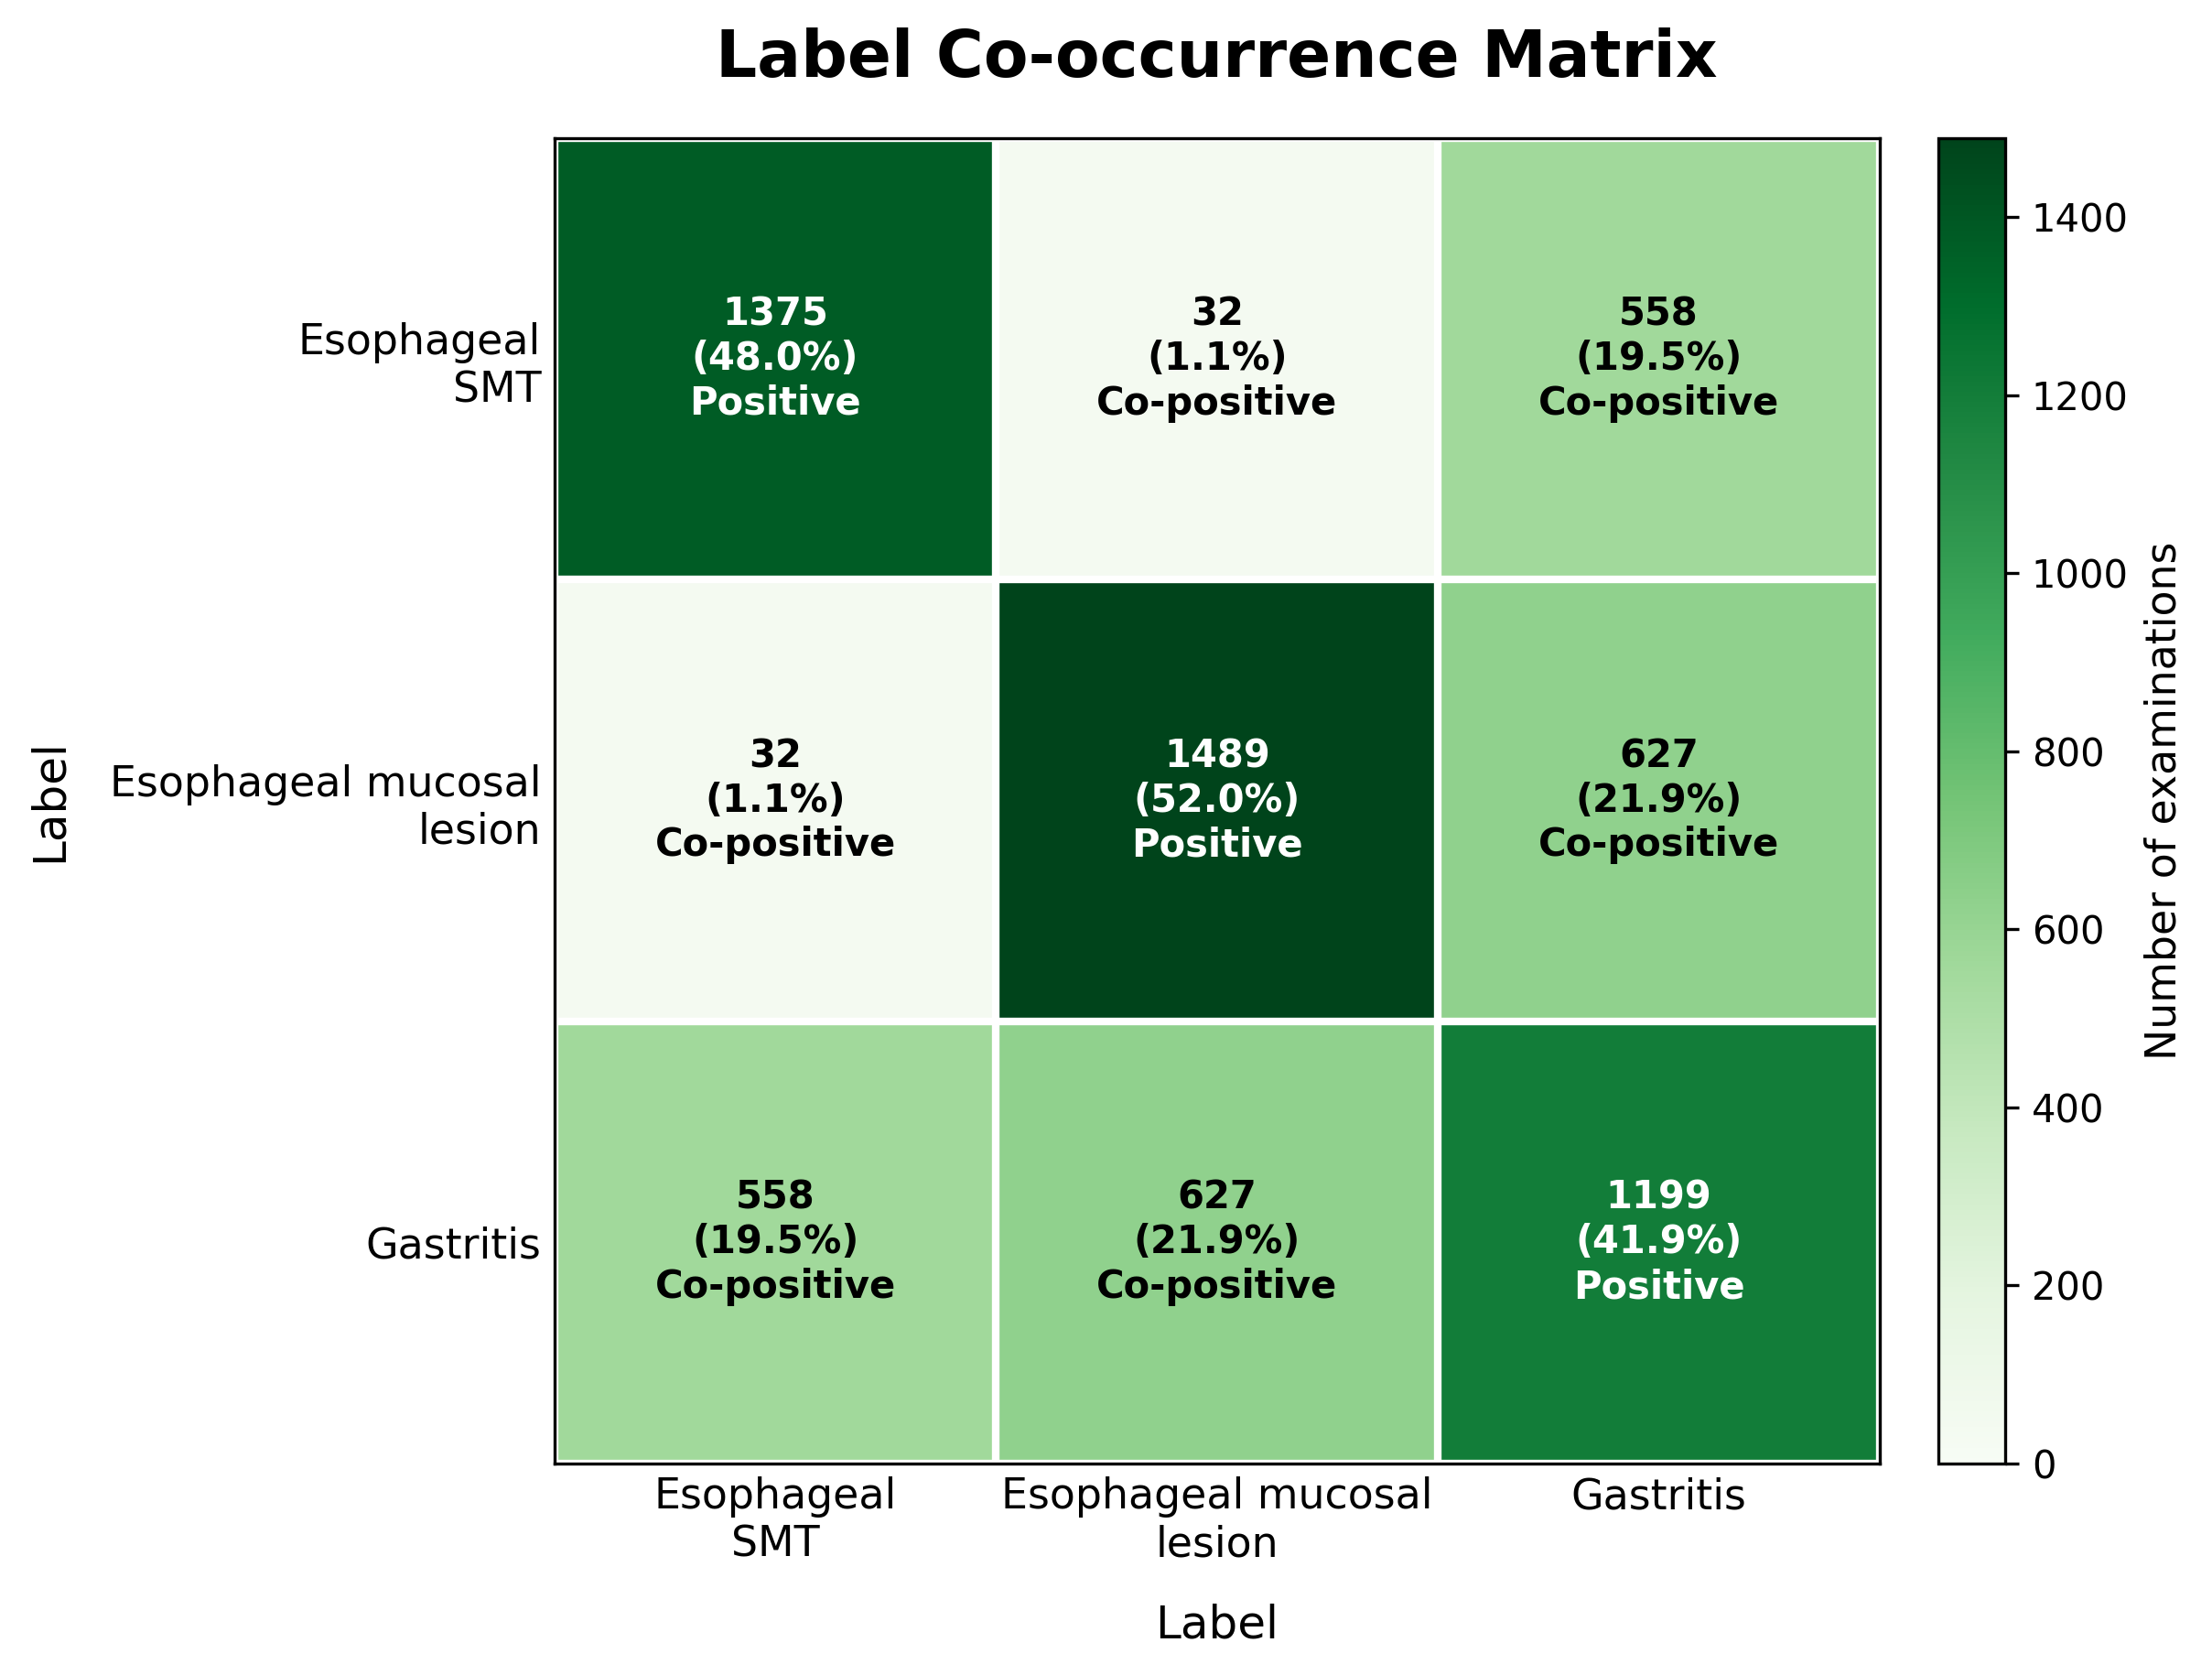
\includegraphics[width=0.74\textwidth]{figs/label_cooccurrence_matrix.png}
\caption{Multi-label co-occurrence matrix of the final study cohort. Diagonal cells show label-positive examinations for each target finding, and off-diagonal cells show pairwise co-positive examinations. Percentages are calculated over all 2863 eligible examinations.\label{fig:label_cooccurrence_matrix}}
\end{figure*}

\subsection{Overall model architecture}
The overall architecture of the proposed \textit{LabelGraph MIL} framework is shown in Figure~\ref{fig:model_structure}. The framework was designed to address four linked requirements of this study: examination-level weak supervision, variable-length multi-image examinations, finding-specific visual evidence aggregation, and dependency modeling among coexisting labels. It consists of four functional layers. First, each gastroscopy examination is represented as a bag of endoscopic images and encoded by a shared ConvNeXt-Tiny instance encoder. Second, label-wise gated attention pooling learns separate attention weights for esophageal submucosal tumor, esophageal mucosal lesion, and gastritis, producing one label-specific representation for each target finding. Third, a learnable label graph reasoner constructs a label-affinity matrix and propagates information among the label-specific representations to model potential coexistence relationships. Finally, independent classification heads transform the refined label representations into examination-level diagnostic probabilities. During training and inference, the framework takes only the image bag of an examination as input; report text is used only to derive training labels and is not provided to the model.

\begin{figure*}[t]
\centering
\includegraphics[width=\textwidth]{figs/model_structure.png}
\caption{Overall modular architecture of the proposed report-guided Label graph MIL framework. A gastroscopy examination is represented as a variable-length image bag and encoded by ConvNeXt-Tiny into instance features. Label-wise gated attention pooling produces finding-specific representations for esophageal submucosal tumor, esophageal mucosal lesion, and gastritis. The label graph reasoner constructs a learnable label-affinity matrix to exchange information among coexisting findings and refines label-specific features before independent classification heads output examination-level diagnostic probabilities.}
\label{fig:model_structure}
\end{figure*}

\textbf{中文翻译：} 本研究提出的\textit{LabelGraph MIL}框架总体结构如图~\ref{fig:model_structure}所示。该框架用于解决本文任务中的四个相互关联的方法学需求：检查级弱监督、变长多图像检查、特定发现的视觉证据聚合，以及共存标签之间的依赖关系建模。整体结构由四个功能层组成。首先，每次胃镜检查被表示为一组内镜图像，并通过共享的ConvNeXt-Tiny实例编码器进行特征提取。其次，标签级门控注意力池化分别为食管黏膜下肿瘤、食管黏膜病变和胃炎学习独立注意力权重，并为每个目标发现生成一个标签特异性表征。第三，可学习标签图推理器构建标签亲和矩阵，并在不同标签特异性表征之间传播信息，以建模潜在共存关系。最后，独立分类头将细化后的标签表征转化为检查级诊断概率。在训练和推理阶段，该框架仅以一次检查对应的图像包作为输入；报告文本仅用于生成训练标签，不作为模型输入。

\textbf{中文翻译：} 图~\ref{fig:model_structure}展示了本文报告引导Label graph MIL框架的模块化总体结构。一次胃镜检查被表示为变长图像包，并由ConvNeXt-Tiny编码为实例特征。标签级门控注意力池化为食管黏膜下肿瘤、食管黏膜病变和胃炎生成特定发现相关表征。标签图推理器构建可学习标签亲和矩阵，在共存发现之间交换信息，并在独立分类头输出检查级诊断概率前细化标签特异性特征。

\subsection{LabelGraph Multiple Instance Learning Framework}
\subsubsection{Examination-level weakly supervised multi-label formulation}
For examination-level multi-label recognition, routine gastroscopy may contain more than one clinically relevant finding, whereas the available supervision is derived from examination reports rather than image-level lesion annotation. Therefore, treating the task as a single-label image classification problem would be inconsistent with both the data structure and the clinical scenario. To address this issue, each examination was defined as one weakly supervised multi-label sample. For the $i$-th examination, the target label was represented as:
\begin{equation}
y_i = [y_{i1},y_{i2},\ldots,y_{iL}] \in \{0,1\}^{L},
\end{equation}
where $L=3$ and the three dimensions correspond to esophageal submucosal tumor, esophageal mucosal lesion, and gastritis. The model estimates an examination-level probability vector:
\begin{equation}
p_i = F_{\Theta}(X_i, M_i) \in [0,1]^{L},
\end{equation}
where $X_i$ denotes the image bag, $M_i$ denotes the corresponding valid-image mask, and $\Theta$ denotes all trainable model parameters. Because the diagnostic conclusion field was used only to generate $y_i$, it was not used as model input. This formulation allows one examination to be positive for multiple labels while avoiding any requirement for image-level lesion boxes, region annotations, or instance labels.

\textbf{中文翻译：} 对于检查级多标签识别问题，常规胃镜检查中可能同时存在多个具有临床意义的发现，而可用监督信号来自检查报告，并非图像级病灶标注。因此，如果将该任务处理为单标签图像分类问题，既不符合数据结构，也不符合临床场景。为解决这一问题，本研究将每次检查定义为一个弱监督多标签样本。对于第$i$次检查，其目标标签表示为：
\begin{equation}
y_i = [y_{i1},y_{i2},\ldots,y_{iL}] \in \{0,1\}^{L},
\end{equation}
其中$L=3$，三个维度分别对应食管黏膜下肿瘤、食管黏膜病变和胃炎。模型估计检查级概率向量：
\begin{equation}
p_i = F_{\Theta}(X_i, M_i) \in [0,1]^{L},
\end{equation}
其中$X_i$表示图像包，$M_i$表示对应的有效图像掩码，$\Theta$表示所有可训练模型参数。由于诊断结论字段仅用于生成$y_i$，因此不作为模型输入。该定义允许同一次检查同时对多个标签呈阳性，同时避免依赖图像级病灶框、区域标注或实例标签。

\subsubsection{Multiple instance learning for variable-length examinations}
For variable-length multi-image examinations, each examination contains a variable number of images, and only a subset of these images may carry evidence for a target finding. Directly forcing all examinations into a single-image representation would discard clinically relevant context, whereas unmasked aggregation of all available images would make the model sensitive to padding, redundant frames, and low-information images. To address this issue, each examination was represented as a multiple-instance bag:
\begin{equation}
X_i=\{I_{i1}, I_{i2}, \ldots, I_{iN_i}\},
\end{equation}
where $N_i$ is the number of images in examination $i$. During mini-batch processing, sampled image bags were padded when necessary, and a binary mask $M_i=\{m_{i1},\ldots,m_{iT}\}$ was used to distinguish valid images from padded or invalid positions:
\begin{equation}
m_{in} =
\begin{cases}
1, & \text{if image position } n \text{ is valid},\\
0, & \text{otherwise}.
\end{cases}
\end{equation}
Each valid image was encoded by a shared instance encoder:
\begin{equation}
h_{in}=f_{\theta}(I_{in}), \quad h_{in}\in \mathbb{R}^{d}.
\end{equation}
In this study, $f_{\theta}$ was implemented using a pretrained ConvNeXt-Tiny backbone followed by a two-layer projection head, which mapped each image to a 512-dimensional instance feature.\cite{R17} The same encoder was shared across all images and target labels.

\textbf{中文翻译：} 对于变长多图像检查问题，每次检查包含的图像数量并不一致，而且只有部分图像可能携带某一目标发现的视觉证据。如果将一次检查强行压缩为单张图像，会丢失具有临床意义的上下文；如果不加区分地聚合所有图像，模型又容易受到填充图像、冗余帧和低信息量图像的影响。为解决这一问题，本研究将每次检查表示为多实例图像包：
\begin{equation}
X_i=\{I_{i1}, I_{i2}, \ldots, I_{iN_i}\},
\end{equation}
其中$N_i$表示第$i$次检查中的图像数量。在小批量处理过程中，采样后的图像包在必要时进行填充，并使用二值掩码$M_i=\{m_{i1},\ldots,m_{iT}\}$区分有效图像与填充或无效位置：
\begin{equation}
m_{in} =
\begin{cases}
1, & \text{若图像位置 } n \text{ 有效},\\
0, & \text{否则}.
\end{cases}
\end{equation}
每张有效图像通过共享实例编码器映射为实例特征：
\begin{equation}
h_{in}=f_{\theta}(I_{in}), \quad h_{in}\in \mathbb{R}^{d}.
\end{equation}
本研究中，$f_{\theta}$由预训练ConvNeXt-Tiny骨干网络和两层投影头实现，将每张图像映射为512维实例特征。该编码器在所有图像和所有目标标签之间共享。

\subsubsection{Masked label-wise attention pooling}
For finding-specific visual evidence aggregation, different findings may depend on different subsets of images. Esophageal submucosal tumor, esophageal mucosal lesion, and gastritis differ in anatomical location and visual appearance; therefore, a single global bag representation shared by all labels may dilute finding-specific evidence. To address this issue, the model learns a separate attention distribution for each target label. Given instance features $H_i=\{h_{i1},\ldots,h_{iT}\}$ and mask $M_i$, the gated attention feature for image $n$ is:
\begin{equation}
q_{in}=\tanh(Vh_{in})\odot\sigma(Uh_{in}),
\end{equation}
where $V$ and $U$ are trainable projections, $\sigma(\cdot)$ is the sigmoid function, and $\odot$ denotes element-wise multiplication. For label $\ell$, the unnormalized attention score is:
\begin{equation}
r_{i\ell n}=w_{\ell}^{\top}q_{in}.
\end{equation}
The mask is incorporated into the attention normalization:
\begin{equation}
a_{i\ell n}=\frac{m_{in}\exp(r_{i\ell n})}{\sum_{t=1}^{T}m_{it}\exp(r_{i\ell t})+\epsilon},
\end{equation}
where $\epsilon$ is a small constant for numerical stability. The label-specific examination representation is then obtained by weighted aggregation:
\begin{equation}
z_{i\ell}=\sum_{n=1}^{T}a_{i\ell n}h_{in}.
\end{equation}
This design allows different labels to attend to different images within the same examination, while padded or invalid image positions are excluded from the aggregation.

\textbf{中文翻译：} 对于特定发现的视觉证据聚合问题，不同目标发现可能依赖不同的图像子集。食管黏膜下肿瘤、食管黏膜病变和胃炎在解剖部位和视觉表现上均存在差异，因此所有标签共享单一全局图像包表征可能会稀释与特定发现相关的证据。为解决这一问题，模型为每个目标标签分别学习注意力分布。给定实例特征$H_i=\{h_{i1},\ldots,h_{iT}\}$和掩码$M_i$，图像$n$的门控注意力特征为：
\begin{equation}
q_{in}=\tanh(Vh_{in})\odot\sigma(Uh_{in}),
\end{equation}
其中$V$和$U$为可训练投影，$\sigma(\cdot)$为sigmoid函数，$\odot$表示逐元素乘法。对于标签$\ell$，未归一化的注意力分数为：
\begin{equation}
r_{i\ell n}=w_{\ell}^{\top}q_{in}.
\end{equation}
模型将掩码纳入注意力归一化过程：
\begin{equation}
a_{i\ell n}=\frac{m_{in}\exp(r_{i\ell n})}{\sum_{t=1}^{T}m_{it}\exp(r_{i\ell t})+\epsilon},
\end{equation}
其中$\epsilon$为用于数值稳定性的小常数。随后，通过加权聚合得到标签特异性检查级表征：
\begin{equation}
z_{i\ell}=\sum_{n=1}^{T}a_{i\ell n}h_{in}.
\end{equation}
该设计使不同标签能够在同一次检查中关注不同图像，同时将填充或无效图像位置排除在聚合过程之外。

\subsubsection{Learnable label graph reasoning}
For dependency modeling among coexisting labels, the three findings are not mutually exclusive. Multiple findings may coexist within the same examination, and completely independent label prediction may fail to use clinically meaningful co-occurrence information. To address this issue, the model performs label graph reasoning after label-wise evidence aggregation. While Figure~\ref{fig:model_structure} presents the complete end-to-end architecture, Figure~\ref{fig:label_graph_reasoner} provides a detailed view of the internal label graph reasoner. The module takes the label-specific representations produced by masked label-wise attention pooling, organizes them as a label-feature matrix, propagates contextual information among the three target labels, and then fuses the propagated context back into the original label-specific evidence through residual refinement. In this way, the graph stage operates as a label-level reasoning module rather than as an additional image encoder or a replacement for label-wise evidence aggregation.

\begin{figure*}[t]
\centering
\includegraphics[width=\textwidth]{figs/label_graph_reasoner.png}
\caption{Detailed structure of the proposed label graph reasoner. The three label-specific feature vectors are concatenated into a label-feature matrix and normalized before graph reasoning. The label graph reasoner propagates information among esophageal submucosal tumor, esophageal mucosal lesion, and gastritis representations, producing label-context features that are combined with the original label-specific features by residual MLP refinement. The loss block indicates the downstream multi-label training objective rather than an additional input to the graph propagation step.\label{fig:label_graph_reasoner}}
\end{figure*}

\textbf{中文翻译：} 对于共存标签之间的依赖关系建模问题，三类目标发现之间并不互斥。同一次检查中可能同时存在多个发现，如果完全独立地预测各标签，可能无法利用具有临床意义的共存信息。为解决这一问题，模型在标签级证据聚合后执行标签图推理。图~\ref{fig:model_structure}展示了端到端总体结构，而图~\ref{fig:label_graph_reasoner}进一步给出了标签图推理器的内部细节。该模块接收由带mask的标签级注意力池化产生的标签特异性表征，将其组织为标签-特征矩阵，在三个目标标签之间传播上下文信息，并通过残差细化将传播后的标签上下文重新融合回原始标签特异性证据。因此，图推理阶段是一个标签级推理模块，而不是额外的图像编码器，也不是对标签级证据聚合的替代。

\textbf{中文翻译：} 图~\ref{fig:label_graph_reasoner}展示了本文标签图推理器的详细结构。三个标签特异性特征向量被拼接为标签-特征矩阵，并在图推理前进行归一化。标签图推理器在食管黏膜下肿瘤、食管黏膜病变和胃炎表征之间传播信息，生成标签上下文特征，并通过残差MLP细化与原始标签特异性特征融合。图中的损失模块表示下游多标签训练目标，而不是图传播步骤的额外输入。

Specifically, let
\begin{equation}
Z_i=[z_{i1},z_{i2},\ldots,z_{iL}]^{\top}\in\mathbb{R}^{L\times d}
\end{equation}
denote the matrix of label-specific examination representations. The model maintains learnable label tokens $E=[e_1,\ldots,e_L]^{\top}\in\mathbb{R}^{L\times d}$, which are row-wise normalized before graph construction:
\begin{equation}
\bar{e}_{\ell}=\frac{e_{\ell}}{\|e_{\ell}\|_2}.
\end{equation}
The label affinity matrix is computed as:
\begin{equation}
A_{\ell k}=\frac{\exp(\bar{e}_{\ell}^{\top}\bar{e}_{k}/\sqrt{d})}{\sum_{r=1}^{L}\exp(\bar{e}_{\ell}^{\top}\bar{e}_{r}/\sqrt{d})}.
\end{equation}
One graph propagation step is then applied to exchange information across label-specific representations:
\begin{equation}
\tilde{Z}_{i}=AZ_i.
\end{equation}
The propagated label context is fused with the original label-specific evidence through residual refinement:
\begin{equation}
Z'_{i}=Z_i+\phi([Z_i;\tilde{Z}_{i}]),
\end{equation}
where $\phi(\cdot)$ is a nonlinear projection implemented by a multilayer perceptron and $[\cdot;\cdot]$ denotes feature concatenation. Finally, each refined label representation is passed to an independent classifier:
\begin{equation}
s_{i\ell}=g_{\ell}(z'_{i\ell}), \quad p_{i\ell}=\sigma(s_{i\ell}),
\end{equation}
where $s_{i\ell}$ is the logit and $p_{i\ell}$ is the predicted probability for label $\ell$. This design preserves label-specific decision boundaries while allowing related labels to exchange contextual information before prediction.

\textbf{中文翻译：} 具体而言，令
\begin{equation}
Z_i=[z_{i1},z_{i2},\ldots,z_{iL}]^{\top}\in\mathbb{R}^{L\times d}
\end{equation}
表示标签特异性检查级表征矩阵。模型维护可学习标签token $E=[e_1,\ldots,e_L]^{\top}\in\mathbb{R}^{L\times d}$，并在构建标签图前对其按行归一化：
\begin{equation}
\bar{e}_{\ell}=\frac{e_{\ell}}{\|e_{\ell}\|_2}.
\end{equation}
标签亲和矩阵计算如下：
\begin{equation}
A_{\ell k}=\frac{\exp(\bar{e}_{\ell}^{\top}\bar{e}_{k}/\sqrt{d})}{\sum_{r=1}^{L}\exp(\bar{e}_{\ell}^{\top}\bar{e}_{r}/\sqrt{d})}.
\end{equation}
随后执行一步标签图传播，使不同标签的特异性表征之间进行信息交换：
\begin{equation}
\tilde{Z}_{i}=AZ_i.
\end{equation}
传播后的标签上下文通过残差细化与原始标签特异性证据进行融合：
\begin{equation}
Z'_{i}=Z_i+\phi([Z_i;\tilde{Z}_{i}]),
\end{equation}
其中$\phi(\cdot)$是由多层感知机实现的非线性投影，$[\cdot;\cdot]$表示特征拼接。最后，每个细化后的标签表征被输入到独立分类器中：
\begin{equation}
s_{i\ell}=g_{\ell}(z'_{i\ell}), \quad p_{i\ell}=\sigma(s_{i\ell}),
\end{equation}
其中$s_{i\ell}$为标签$\ell$的logit，$p_{i\ell}$为对应预测概率。该设计在保留各标签独立决策边界的同时，使相关标签在预测前能够交换上下文信息。

\section{Experiments}

\subsection{Experimental Settings}
All experiments used the same training, validation, and test split described in Table~\ref{T1}. Model selection was performed on the validation set using macro F1, and all reported results were measured on the fixed internal test set. Macro F1 was used as the primary evaluation metric because the task was a three-label examination-level classification problem with non-mutually exclusive labels. Micro F1, macro ROC-AUC, macro PR-AUC, subset accuracy, hamming loss, and Cohen's kappa were also reported to characterize overall discrimination, exact multi-label agreement, and prediction consistency.\cite{R18} Unless otherwise specified, all experiments followed the same preprocessing, training, checkpoint selection, and test-time decision threshold.

In implementation, all input images were resized to 224$\times$224 pixels. Each mini-batch contained 12 examinations, and each examination was represented by at most 16 sampled images during both training and evaluation; therefore, one mini-batch contained at most 192 image instances. For examinations with fewer sampled images, padding was used, and a binary valid-image mask ensured that padded positions did not contribute to attention pooling or downstream loss computation. Random instance sampling was used during training to expose the model to different image subsets, whereas uniform sampling was used during validation and testing to provide deterministic examination-level evaluation. The model used a ConvNeXt-Tiny backbone, a 512-dimensional projected instance feature, an attention dimension of 256, and a dropout rate of 0.2. Training was performed for up to 30 epochs with AdamW,\cite{R19} an initial learning rate of $2\times10^{-5}$, weight decay of 0.02, a warm-up ratio of 0.2, mixed-precision training, and asymmetric loss for multi-label optimization.\cite{R20} A random instance dropout rate of 0.25 was used as regularization to reduce over-reliance on a small subset of frames.

\textbf{中文翻译：} 所有实验均使用表~\ref{T1}所示的相同训练集、验证集和测试集划分。模型选择基于验证集宏平均F1，所有结果均在固定内部测试集上报告。由于本研究是三标签检查级多标签分类任务，且标签之间并不互斥，因此将宏平均F1作为主要评价指标。同时报告微平均F1、宏平均ROC-AUC、宏平均PR-AUC、子集准确率、汉明损失和Cohen's kappa，以反映整体判别能力、严格多标签一致性和预测一致性。除非特别说明，所有实验均采用相同的预处理、训练流程、checkpoint选择规则和测试阶段判定阈值。

\textbf{中文翻译：} 在具体实现中，所有输入图像均被缩放至224$\times$224像素。每个mini-batch包含12次检查，每次检查在训练和评估阶段最多采样16张图像，因此一个mini-batch中最多包含192个图像实例。对于采样图像数不足的检查，使用padding补齐，并通过二值有效图像mask保证填充位置不参与注意力池化和下游损失计算。训练阶段使用随机实例采样，使模型能够接触同一次检查中的不同图像子集；验证和测试阶段使用均匀采样，以保证检查级评估的确定性。模型采用ConvNeXt-Tiny骨干网络，实例特征投影维度为512，注意力维度为256，dropout为0.2。训练最多进行30个epoch，优化器为AdamW，初始学习率为$2\times10^{-5}$，权重衰减为0.02，warm-up比例为0.2，并使用混合精度训练和适用于多标签优化的asymmetric loss。随机实例dropout设置为0.25，用于降低模型对少数图像帧的过度依赖。

\subsection{Overall model comparison}
To determine whether the proposed framework improves clinically relevant examination-level multi-label classification beyond standard aggregation strategies and representative weakly supervised MIL methods, we conducted a broad model comparison experiment. The design included five baseline MIL models and five adapted state-of-the-art MIL models, all evaluated under the same internal test protocol as the proposed model. Because the intended use is multi-label examination triage rather than single-image diagnosis, the comparison reports both threshold-dependent metrics, including macro F1, micro F1, subset accuracy, hamming loss, and Cohen's kappa, and ranking-based metrics, including macro ROC-AUC and macro PR-AUC.

\textbf{中文翻译：} 为了判断本文框架相对于标准检查级聚合策略和代表性弱监督MIL方法是否能够提升具有临床意义的检查级多标签分类性能，我们进行了全面的模型对比实验。实验设计纳入五种基础MIL模型和五种改造后的先进MIL模型，并将它们与本文模型置于相同内部测试流程下评估。由于本研究面向多标签检查级分诊，而不是单图像诊断，表中同时报告阈值相关指标，包括宏平均F1、微平均F1、子集准确率、汉明损失和Cohen's kappa，以及排序型指标，包括宏平均ROC-AUC和宏平均PR-AUC。

The compared models were selected to cover both simple MIL aggregation rules and published weakly supervised MIL architectures. Attention MIL, CLAM-MB, CLAM-SB, DSMIL, TransMIL, and DTFD-MIL follow the corresponding methods introduced in the related work section and were adapted from their original bag-level settings to the present three-label gastroscopy task. Mean pooling and max pooling were included as non-parametric aggregation baselines to test whether learned evidence weighting was necessary. Transformer-context MIL used the Transformer self-attention block as an instance-context aggregation module,\cite{R21} whereas Top-$k$ MIL followed the top-ranked instance selection strategy used in weakly supervised computational pathology.\cite{R22} The proposed Label graph MIL differs from these baselines by combining label-wise evidence aggregation with explicit label relation reasoning.

\textbf{中文翻译：} 对比模型的选择覆盖了简单MIL聚合规则和已发表的弱监督MIL结构。Attention MIL、CLAM-MB、CLAM-SB、DSMIL、TransMIL和DTFD-MIL均对应相关工作部分已介绍的方法，并从其原始包级任务设置适配到本文三标签胃镜任务。Mean pooling和max pooling作为非参数聚合基线，用于检验是否需要可学习的证据加权。Transformer-context MIL使用Transformer自注意力模块进行实例上下文聚合，而Top-$k$ MIL参考弱监督计算病理中的高排名实例选择策略。本文提出的Label graph MIL则与上述基线不同，它将标签级证据聚合与显式标签关系推理结合起来。

\begin{table*}[t]
\scriptsize\sf\centering
\caption{Overall comparison with baseline and adapted state-of-the-art MIL models on the internal test set.\label{T2}}
\resizebox{\textwidth}{!}{%
\begin{tabular}{ll*{9}{c}}
\toprule
Group & Model & \shortstack{Macro\\Recall} & \shortstack{Macro\\Precision} & \shortstack{Macro\\F1} & \shortstack{Macro\\ROC-AUC} & \shortstack{Macro\\PR-AUC} & \shortstack{Subset\\accuracy} & \shortstack{Hamming\\loss} & Kappa & \shortstack{Mean\\$p$-value} \\
\midrule
Proposed & Label graph MIL & \shortstack{0.9015\\{[}0.8807, 0.9213{]}} & \shortstack{\textbf{0.8340}\\{[}0.8126, 0.8547{]}} & \shortstack{\textbf{0.8650}\\{[}0.8460, 0.8826{]}} & \shortstack{0.9187\\{[}0.9008, 0.9358{]}} & \shortstack{0.9106\\{[}0.8912, 0.9320{]}} & \shortstack{0.7021\\{[}0.6638, 0.7404{]}} & \shortstack{\textbf{0.1400}\\{[}0.1208, 0.1597{]}} & \shortstack{\textbf{0.7206}\\{[}0.6811, 0.7587{]}} & 1.0000 \\
\midrule
Baseline & Attention MIL & \shortstack{0.8895\\{[}0.8683, 0.9110{]}} & \shortstack{0.8170\\{[}0.7946, 0.8391{]}} & \shortstack{0.8504\\{[}0.8308, 0.8692{]}} & \shortstack{0.9179\\{[}0.9001, 0.9353{]}} & \shortstack{0.9164\\{[}0.8982, 0.9350{]}} & \shortstack{0.6672\\{[}0.6289, 0.7073{]}} & \shortstack{0.1556\\{[}0.1353, 0.1760{]}} & \shortstack{0.6894\\{[}0.6490, 0.7299{]}} & 0.1906 \\
Baseline & Mean pooling & \shortstack{0.9131\\{[}0.8951, 0.9308{]}} & \shortstack{0.8119\\{[}0.7903, 0.8332{]}} & \shortstack{0.8584\\{[}0.8404, 0.8762{]}} & \shortstack{0.9190\\{[}0.9019, 0.9363{]}} & \shortstack{0.9102\\{[}0.8899, 0.9309{]}} & \shortstack{0.6742\\{[}0.6359, 0.7143{]}} & \shortstack{0.1487\\{[}0.1289, 0.1678{]}} & \shortstack{0.7035\\{[}0.6652, 0.7427{]}} & 0.3786 \\
Baseline & Transformer-context MIL & \shortstack{0.9036\\{[}0.8839, 0.9237{]}} & \shortstack{0.8195\\{[}0.7970, 0.8395{]}} & \shortstack{0.8589\\{[}0.8404, 0.8757{]}} & \shortstack{\textbf{0.9253}\\{[}0.9089, 0.9412{]}} & \shortstack{\textbf{0.9181}\\{[}0.8995, 0.9370{]}} & \shortstack{0.6812\\{[}0.6411, 0.7178{]}} & \shortstack{0.1475\\{[}0.1289, 0.1678{]}} & \shortstack{0.7057\\{[}0.6653, 0.7429{]}} & 0.3370 \\
Baseline & Top-$k$ MIL & \shortstack{0.9182\\{[}0.8993, 0.9349{]}} & \shortstack{0.8124\\{[}0.7915, 0.8340{]}} & \shortstack{0.8606\\{[}0.8431, 0.8767{]}} & \shortstack{0.9220\\{[}0.9044, 0.9389{]}} & \shortstack{0.9106\\{[}0.8901, 0.9316{]}} & \shortstack{0.6620\\{[}0.6254, 0.7038{]}} & \shortstack{0.1487\\{[}0.1301, 0.1678{]}} & \shortstack{0.7037\\{[}0.6660, 0.7409{]}} & 0.3044 \\
Baseline & Max pooling & \shortstack{\textbf{0.9668}\\{[}0.9550, 0.9780{]}} & \shortstack{0.6261\\{[}0.6094, 0.6420{]}} & \shortstack{0.7533\\{[}0.7412, 0.7648{]}} & \shortstack{0.8439\\{[}0.8246, 0.8638{]}} & \shortstack{0.8416\\{[}0.8204, 0.8652{]}} & \shortstack{0.1533\\{[}0.1237, 0.1812{]}} & \shortstack{0.3287\\{[}0.3136, 0.3438{]}} & \shortstack{0.3544\\{[}0.3246, 0.3826{]}} & $<$0.001 \\
\midrule
Adapted SOTA & TransMIL & \shortstack{0.8928\\{[}0.8712, 0.9119{]}} & \shortstack{0.8309\\{[}0.8096, 0.8542{]}} & \shortstack{0.8606\\{[}0.8411, 0.8800{]}} & \shortstack{0.9247\\{[}0.9076, 0.9407{]}} & \shortstack{0.9179\\{[}0.9011, 0.9366{]}} & \shortstack{\textbf{0.7143}\\{[}0.6794, 0.7526{]}} & \shortstack{0.1429\\{[}0.1220, 0.1632{]}} & \shortstack{0.7147\\{[}0.6740, 0.7564{]}} & 0.5912 \\
Adapted SOTA & DSMIL & \shortstack{0.9010\\{[}0.8826, 0.9199{]}} & \shortstack{0.8238\\{[}0.8030, 0.8462{]}} & \shortstack{0.8601\\{[}0.8424, 0.8781{]}} & \shortstack{0.9241\\{[}0.9075, 0.9407{]}} & \shortstack{\textbf{0.9181}\\{[}0.8998, 0.9372{]}} & \shortstack{0.6951\\{[}0.6585, 0.7334{]}} & \shortstack{0.1452\\{[}0.1249, 0.1643{]}} & \shortstack{0.7102\\{[}0.6721, 0.7506{]}} & 0.5150 \\
Adapted SOTA & DTFD-MIL & \shortstack{0.9378\\{[}0.9215, 0.9527{]}} & \shortstack{0.7716\\{[}0.7529, 0.7904{]}} & \shortstack{0.8452\\{[}0.8305, 0.8600{]}} & \shortstack{0.9177\\{[}0.9009, 0.9340{]}} & \shortstack{0.9098\\{[}0.8916, 0.9299{]}} & \shortstack{0.5714\\{[}0.5314, 0.6115{]}} & \shortstack{0.1719\\{[}0.1539, 0.1899{]}} & \shortstack{0.6583\\{[}0.6220, 0.6936{]}} & 0.1999 \\
Adapted SOTA & CLAM-MB & \shortstack{0.9025\\{[}0.8831, 0.9223{]}} & \shortstack{0.7803\\{[}0.7597, 0.8015{]}} & \shortstack{0.8360\\{[}0.8188, 0.8526{]}} & \shortstack{0.9071\\{[}0.8895, 0.9238{]}} & \shortstack{0.9000\\{[}0.8795, 0.9213{]}} & \shortstack{0.5958\\{[}0.5575, 0.6359{]}} & \shortstack{0.1760\\{[}0.1574, 0.1951{]}} & \shortstack{0.6496\\{[}0.6109, 0.6867{]}} & 0.1308 \\
Adapted SOTA & CLAM-SB & \shortstack{0.9219\\{[}0.9043, 0.9387{]}} & \shortstack{0.7550\\{[}0.7349, 0.7769{]}} & \shortstack{0.8284\\{[}0.8122, 0.8445{]}} & \shortstack{0.9070\\{[}0.8889, 0.9247{]}} & \shortstack{0.8907\\{[}0.8682, 0.9152{]}} & \shortstack{0.5453\\{[}0.5070, 0.5871{]}} & \shortstack{0.1911\\{[}0.1719, 0.2096{]}} & \shortstack{0.6203\\{[}0.5838, 0.6589{]}} & 0.0151 \\
\bottomrule
\end{tabular}
}
\end{table*}

As shown in Table~\ref{T2}, the proposed Label graph MIL achieved the best macro F1 (0.8650), micro F1 (0.8616), hamming loss (0.1400), and Cohen's kappa (0.7206). These results indicate that the proposed model was strongest on the primary F1-based decision metrics and produced the most consistent multi-label predictions among the compared methods. The improvement over the strongest non-proposed F1 result was modest but consistent, suggesting that label-wise evidence aggregation combined with label relation reasoning improves the final thresholded decision rather than merely changing probability calibration. Transformer-context MIL and DSMIL reached the highest macro ROC-AUC or macro PR-AUC, and TransMIL achieved the highest subset accuracy, indicating that instance-context modeling and transformer-based MIL remain strong comparators for probability ranking or exact-set prediction. However, the proposed model provided the best overall balance for the main task objective, especially when macro F1 and kappa are considered together.

\textbf{中文翻译：} 如表~\ref{T2}所示，本文Label graph MIL在宏平均F1（0.8650）、微平均F1（0.8616）、汉明损失（0.1400）和Cohen's kappa（0.7206）上取得最佳结果。这说明本文模型在以F1为核心的主要判定指标上表现最强，并在所有对比方法中产生了最一致的多标签预测。相对于非本文模型中的最佳F1结果，本文模型的提升幅度并不夸张但较为稳定，提示标签级证据聚合与标签关系推理的结合能够改善最终阈值判定，而不仅仅是改变概率校准。Transformer-context MIL和DSMIL在宏平均ROC-AUC或宏平均PR-AUC上取得最高值，TransMIL在子集准确率上取得最高值，说明实例上下文建模和Transformer类MIL在概率排序或严格标签集合预测方面仍是较强对照。然而，结合宏平均F1和kappa来看，本文模型对本研究的主要任务目标提供了更好的整体平衡。

Overall, this experiment supports the proposed Label graph MIL as the primary model for examination-level multi-label gastroscopy classification, while also showing that different MIL designs emphasize different evaluation aspects.

\textbf{中文翻译：} 总体而言，该实验支持将本文Label graph MIL作为检查级多标签胃镜分类的主模型，同时也说明不同MIL结构会偏向不同评价指标。

\subsection{Label-wise performance}
To examine whether the overall performance of the proposed model was shared across all target findings rather than being dominated by one easier label, we conducted a label-wise evaluation experiment. This analysis is important in the weakly supervised examination-level setting because localized esophageal abnormalities and diffuse gastric inflammatory changes may generate different visual evidence patterns. The primary checkpoint was therefore evaluated separately for esophageal submucosal tumor, esophageal mucosal lesion, and gastritis using recall, precision, F1, ROC-AUC, and PR-AUC.

\textbf{中文翻译：} 为了分析本文模型的整体性能是否来自三个目标发现的共同贡献，而不是被某一个相对容易的标签主导，我们进行了分标签评估实验。该分析在检查级弱监督场景中尤为重要，因为局灶性食管异常和弥漫性胃黏膜炎症可能对应不同的视觉证据模式。因此，本研究分别从召回率、精确率、F1、ROC-AUC和PR-AUC评估主模型checkpoint在食管黏膜下肿瘤、食管黏膜病变和胃炎三个标签上的表现。

\begin{table*}[t]
\footnotesize\sf\centering
\caption{Label-wise internal test performance of the proposed model.\label{T3}}
\resizebox{\textwidth}{!}{%
\begin{tabular}{p{0.34\textwidth}ccccc}
\toprule
Label & Recall & Precision & F1 & ROC-AUC & PR-AUC \\
\midrule
Esophageal submucosal tumor & \shortstack{0.9239\\{[}0.8904, 0.9536{]}} & \shortstack{0.7727\\{[}0.7264, 0.8198{]}} & \shortstack{0.8416\\{[}0.8082, 0.8726{]}} & \shortstack{0.8932\\{[}0.8661, 0.9184{]}} & \shortstack{0.8553\\{[}0.8081, 0.9028{]}} \\
Esophageal mucosal lesion & \shortstack{0.8700\\{[}0.8289, 0.9072{]}} & \shortstack{0.8006\\{[}0.7564, 0.8439{]}} & \shortstack{0.8339\\{[}0.8014, 0.8645{]}} & \shortstack{0.9028\\{[}0.8761, 0.9275{]}} & \shortstack{0.9263\\{[}0.9055, 0.9465{]}} \\
Gastritis & \shortstack{0.9105\\{[}0.8745, 0.9438{]}} & \shortstack{0.9286\\{[}0.8941, 0.9585{]}} & \shortstack{0.9194\\{[}0.8938, 0.9425{]}} & \shortstack{0.9602\\{[}0.9422, 0.9768{]}} & \shortstack{0.9502\\{[}0.9243, 0.9726{]}} \\
\bottomrule
\end{tabular}
}
\end{table*}

Table~\ref{T3} shows that gastritis had the strongest label-wise performance, with an F1 of 0.9194, ROC-AUC of 0.9602, and PR-AUC of 0.9502. This result suggests that the model can reliably aggregate evidence for gastric inflammatory changes, which are often more spatially distributed across an examination. The two esophageal labels remained clinically meaningful but were more challenging: esophageal submucosal tumor achieved high recall (0.9239) but lower precision (0.7727), whereas esophageal mucosal lesion had a more balanced recall-precision profile and a higher PR-AUC (0.9263). These differences suggest that examination-level weak supervision can capture sparse esophageal evidence, but distinguishing localized esophageal abnormalities remains harder than identifying gastritis.

\textbf{中文翻译：} 表~\ref{T3}显示，胃炎标签取得最强的分标签表现，其F1为0.9194，ROC-AUC为0.9602，PR-AUC为0.9502。这一结果提示模型能够较可靠地聚合胃黏膜炎症相关证据，而此类证据往往在一次检查中分布更广。两个食管相关标签仍具有较好的临床可用表现，但识别难度更高：食管黏膜下肿瘤召回率较高（0.9239），但精确率相对较低（0.7727）；食管黏膜病变的召回率和精确率更加均衡，并取得较高的PR-AUC（0.9263）。这些差异说明，检查级弱监督能够捕获稀疏的食管相关证据，但局灶性食管异常的区分仍比胃炎识别更具挑战性。

To further visualize the test-set behavior of the proposed model, we plotted the label-wise confusion matrices and the corresponding ROC and PR curves. Figure~\ref{fig:test_confusion_matrix} presents the thresholded binary decisions for each target finding. The diagonal cells indicate correctly classified negative and positive examinations, whereas the off-diagonal cells correspond to false positives and false negatives. The model detected most positive examinations for all three labels, with 255 true positives for esophageal submucosal tumor, 261 for esophageal mucosal lesion, and 234 for gastritis. The gastritis matrix showed the most balanced error profile, with only 18 false positives and 23 false negatives, which is consistent with its highest F1 and precision in Table~\ref{T3}. In contrast, the two esophageal findings had more false-positive predictions, especially esophageal submucosal tumor. This suggests that the model was sensitive to esophageal abnormalities but may assign positive predictions to some visually ambiguous or nonspecific esophageal frames, explaining the lower precision of the esophageal labels.

\textbf{中文翻译：} 为了进一步可视化本文模型在测试集上的表现，我们绘制了分标签混淆矩阵以及对应的ROC和PR曲线。图~\ref{fig:test_confusion_matrix}展示了每个目标发现的阈值化二分类结果。对角线单元格表示被正确分类的阴性和阳性检查，非对角线单元格分别对应假阳性和假阴性。模型能够识别三个标签中大部分阳性检查，其中食管黏膜下肿瘤真阳性为255例，食管黏膜病变真阳性为261例，胃炎真阳性为234例。胃炎的混淆矩阵呈现出最均衡的错误模式，仅有18例假阳性和23例假阴性，这与表~\ref{T3}中胃炎取得最高F1和精确率的结果一致。相比之下，两个食管相关发现出现了更多假阳性预测，尤其是食管黏膜下肿瘤。这提示模型对食管异常具有较高敏感性，但对于部分视觉表现不明确或非特异性的食管图像，仍可能给出阳性预测，从而解释了食管相关标签精确率相对较低的现象。

Figure~\ref{fig:test_roc_pr_curve} further characterizes the score-ranking behavior before applying a fixed decision threshold. The ROC curves show that the model separated positive and negative examinations well across a wide range of thresholds, with ROC-AUC values of 0.8932, 0.9028, and 0.9602 for esophageal submucosal tumor, esophageal mucosal lesion, and gastritis, respectively. The PR curves are particularly informative for this multi-label setting because they directly reflect the precision-recall trade-off for each finding. Gastritis maintained the highest PR-AUC, indicating stable precision even when recall was high. Esophageal mucosal lesion also showed strong PR performance, whereas esophageal submucosal tumor had a lower PR-AUC, matching the larger number of false positives observed in Figure~\ref{fig:test_confusion_matrix}. Together, these visualizations complement Table~\ref{T3} by showing both the final thresholded decision pattern and the underlying ranking quality of the proposed model.

\textbf{中文翻译：} 图~\ref{fig:test_roc_pr_curve}进一步展示了模型在应用固定判定阈值之前的分数排序行为。ROC曲线显示，模型在较宽阈值范围内均能较好地区分阳性和阴性检查，食管黏膜下肿瘤、食管黏膜病变和胃炎的ROC-AUC分别为0.8932、0.9028和0.9602。PR曲线对于本研究的多标签场景尤其重要，因为它直接反映了每个目标发现的精确率-召回率权衡。胃炎取得最高PR-AUC，说明在保持较高召回率时仍能维持稳定精确率。食管黏膜病变同样表现出较强的PR性能，而食管黏膜下肿瘤的PR-AUC相对较低，这与图~\ref{fig:test_confusion_matrix}中其假阳性数量较多的现象一致。综合来看，这些可视化结果从最终阈值化判定模式和模型底层排序质量两个方面补充了表~\ref{T3}中的分标签数值结果。

\begin{figure*}[t]
\centering
\includegraphics[width=\textwidth]{figs/confusion_matrix.png}
\caption{Label-wise confusion matrices of the proposed model on the internal test set. Each matrix shows thresholded binary decisions for one target finding, with rows indicating true labels and columns indicating predicted labels. Diagonal cells represent correctly classified examinations, whereas off-diagonal cells represent false-positive and false-negative predictions.\label{fig:test_confusion_matrix}}
\end{figure*}

\begin{figure*}[t]
\centering
\includegraphics[width=\textwidth]{figs/roc_pr_curve.png}
\caption{Label-wise ROC and PR curves of the proposed model on the internal test set. The ROC curves show discrimination performance across thresholds, and the PR curves summarize the precision-recall trade-off for the three target findings. The values in the legends correspond to the label-wise ROC-AUC and PR-AUC reported in Table~\ref{T3}.\label{fig:test_roc_pr_curve}}
\end{figure*}

In summary, the label-wise results indicate that the proposed model is not driven by a single easy label; rather, it maintains useful performance across all three findings while showing the expected difficulty gradient between diffuse and localized endoscopic abnormalities.

\textbf{中文翻译：} 总体来看，分标签结果表明本文模型并非仅依赖单一容易标签取得平均性能，而是在三个目标发现上均保持了有效表现，同时呈现出弥漫性异常与局灶性异常之间符合预期的难度差异。

\subsection{Ablation of label relation reasoning}
To verify whether label relation reasoning provides independent value beyond label-wise evidence aggregation, we conducted a module-effect ablation experiment. The design was based on the clinical fact that the three target findings are not mutually exclusive, so label-specific representations may benefit from exchanging contextual information before prediction. We therefore compared the proposed learnable label graph reasoner with a no-graph variant and several alternative label interaction modules, including attention-based, graph-based, and feature-mixing designs. All variants retained the same upstream image encoder and label-wise evidence aggregation, allowing the comparison to focus on the label interaction stage.

\textbf{中文翻译：} 为了验证标签关系推理是否能够在标签级证据聚合之外提供独立贡献，我们进行了模块作用消融实验。该实验设计基于三个目标发现并不互斥这一临床事实，因此标签特异性表征可能受益于预测前的上下文信息交换。本文将可学习标签图推理器与去除标签图的变体以及多种替代标签交互模块进行比较，包括基于注意力、基于图和基于特征混合的设计。所有变体均保留相同的上游图像编码器和标签级证据聚合，使比较能够聚焦于标签交互阶段。

The modules in Table~\ref{T4} were organized according to their structural origins. Full Label Graph is the proposed reasoner, inspired by label-graph dependency modeling in multi-label recognition but redesigned for label-wise MIL representations. The no-graph variant removes this interaction stage and directly classifies each label-specific embedding. Label Self-Attention Reasoner and Label Transformer Reasoner are attention/sequence variants based on the Transformer self-attention mechanism already cited above. Dynamic Label GAT Reasoner follows the graph attention network idea,\cite{R23} Cosine Dynamic Graph Reasoner follows pairwise affinity modeling similar to non-local neural operations,\cite{R24} and Static Co-occurrence GCN Reasoner follows graph convolutional propagation on a fixed graph.\cite{R25} Low-Rank Label Graph Reasoner uses a low-rank factorized interaction design related to factorized bilinear pooling,\cite{R26} whereas Label MLP-Mixer Reasoner adapts the token-mixing idea of MLP-Mixer to label embeddings.\cite{R27}

\textbf{中文翻译：} 表~\ref{T4}中的模块按照其结构来源进行组织。Full Label Graph是本文提出的推理器，其设计受到多标签识别中标签图依赖建模思想的启发，但被重新设计用于标签级MIL表征。无标签图变体删除标签交互阶段，并直接对每个标签特异性嵌入进行分类。Label Self-Attention Reasoner和Label Transformer Reasoner属于注意力/序列建模变体，基于前文已引用的Transformer自注意力机制。Dynamic Label GAT Reasoner参考图注意力网络思想，Cosine Dynamic Graph Reasoner参考类似non-local神经操作的成对亲和建模，Static Co-occurrence GCN Reasoner参考固定图上的图卷积传播。Low-Rank Label Graph Reasoner使用与因子化双线性池化相关的低秩交互设计，而Label MLP-Mixer Reasoner则将MLP-Mixer中的token mixing思想适配到标签嵌入交互中。

\begin{table*}[h]
\scriptsize\sf\centering
\caption{Module-effect ablation of label relation reasoners on the internal test set.\label{T4}}
\resizebox{\textwidth}{!}{%
\begin{tabular}{ll*{9}{c}}
\toprule
Module & Category & \shortstack{Macro\\Recall} & \shortstack{Macro\\Precision} & \shortstack{Macro\\F1} & \shortstack{Macro\\ROC-AUC} & \shortstack{Macro\\PR-AUC} & \shortstack{Subset\\accuracy} & \shortstack{Hamming\\loss} & Kappa & \shortstack{Mean\\$p$-value} \\
\midrule
Full Label Graph & Proposed & \shortstack{0.9015\\{[}0.8807, 0.9213{]}} & \shortstack{\textbf{0.8340}\\{[}0.8126, 0.8547{]}} & \shortstack{\textbf{0.8650}\\{[}0.8460, 0.8826{]}} & \shortstack{0.9187\\{[}0.9008, 0.9358{]}} & \shortstack{0.9106\\{[}0.8912, 0.9320{]}} & \shortstack{0.7021\\{[}0.6638, 0.7404{]}} & \shortstack{\textbf{0.1400}\\{[}0.1208, 0.1597{]}} & \shortstack{\textbf{0.7206}\\{[}0.6811, 0.7587{]}} & 1.0000 \\
w/o Label Graph Reasoner & Removal & \shortstack{\textbf{0.9409}\\{[}0.9252, 0.9558{]}} & \shortstack{0.7854\\{[}0.7657, 0.8051{]}} & \shortstack{0.8539\\{[}0.8384, 0.8682{]}} & \shortstack{0.9252\\{[}0.9085, 0.9413{]}} & \shortstack{\textbf{0.9211}\\{[}0.9027, 0.9387{]}} & \shortstack{0.6010\\{[}0.5627, 0.6429{]}} & \shortstack{0.1626\\{[}0.1440, 0.1806{]}} & \shortstack{0.6767\\{[}0.6402, 0.7131{]}} & 0.0284 \\
Label Self-Attention Reasoner & Attention/sequence & \shortstack{0.9067\\{[}0.8878, 0.9247{]}} & \shortstack{0.8113\\{[}0.7904, 0.8329{]}} & \shortstack{0.8560\\{[}0.8383, 0.8729{]}} & \shortstack{0.9201\\{[}0.9036, 0.9365{]}} & \shortstack{0.9085\\{[}0.8900, 0.9292{]}} & \shortstack{0.6707\\{[}0.6341, 0.7091{]}} & \shortstack{0.1516\\{[}0.1324, 0.1707{]}} & \shortstack{0.6977\\{[}0.6595, 0.7362{]}} & 0.3298 \\
Label Transformer Reasoner & Attention/sequence & \shortstack{0.8901\\{[}0.8705, 0.9105{]}} & \shortstack{0.8234\\{[}0.8024, 0.8452{]}} & \shortstack{0.8547\\{[}0.8372, 0.8734{]}} & \shortstack{0.9183\\{[}0.9006, 0.9347{]}} & \shortstack{0.9090\\{[}0.8889, 0.9284{]}} & \shortstack{0.6864\\{[}0.6498, 0.7247{]}} & \shortstack{0.1504\\{[}0.1301, 0.1690{]}} & \shortstack{0.6997\\{[}0.6622, 0.7402{]}} & 0.3778 \\
Dynamic Label GAT Reasoner & Graph variants & \shortstack{0.9247\\{[}0.9073, 0.9416{]}} & \shortstack{0.8124\\{[}0.7920, 0.8332{]}} & \shortstack{0.8636\\{[}0.8467, 0.8800{]}} & \shortstack{\textbf{0.9259}\\{[}0.9094, 0.9424{]}} & \shortstack{0.9202\\{[}0.9016, 0.9386{]}} & \shortstack{0.6655\\{[}0.6254, 0.7056{]}} & \shortstack{0.1458\\{[}0.1266, 0.1649{]}} & \shortstack{0.7095\\{[}0.6717, 0.7477{]}} & 0.2971 \\
Cosine Dynamic Graph Reasoner & Graph variants & \shortstack{0.9092\\{[}0.8907, 0.9271{]}} & \shortstack{0.8232\\{[}0.8014, 0.8460{]}} & \shortstack{0.8636\\{[}0.8458, 0.8814{]}} & \shortstack{0.9187\\{[}0.9021, 0.9353{]}} & \shortstack{0.9081\\{[}0.8873, 0.9298{]}} & \shortstack{0.7003\\{[}0.6620, 0.7387{]}} & \shortstack{0.1417\\{[}0.1225, 0.1614{]}} & \shortstack{0.7173\\{[}0.6785, 0.7556{]}} & 0.7171 \\
Static Co-occurrence GCN Reasoner & Graph variants & \shortstack{0.9079\\{[}0.8891, 0.9264{]}} & \shortstack{0.8230\\{[}0.8008, 0.8453{]}} & \shortstack{0.8629\\{[}0.8442, 0.8801{]}} & \shortstack{0.9191\\{[}0.9021, 0.9357{]}} & \shortstack{0.9089\\{[}0.8880, 0.9304{]}} & \shortstack{0.7003\\{[}0.6620, 0.7387{]}} & \shortstack{0.1423\\{[}0.1231, 0.1620{]}} & \shortstack{0.7161\\{[}0.6769, 0.7543{]}} & 0.7007 \\
Low-Rank Label Graph Reasoner & Graph variants & \shortstack{0.8801\\{[}0.8572, 0.8999{]}} & \shortstack{0.8242\\{[}0.8009, 0.8469{]}} & \shortstack{0.8506\\{[}0.8297, 0.8697{]}} & \shortstack{0.9160\\{[}0.8979, 0.9330{]}} & \shortstack{0.9108\\{[}0.8918, 0.9308{]}} & \shortstack{0.6882\\{[}0.6498, 0.7265{]}} & \shortstack{0.1521\\{[}0.1318, 0.1731{]}} & \shortstack{0.6961\\{[}0.6540, 0.7364{]}} & 0.2763 \\
Label MLP-Mixer Reasoner & Feature mixer & \shortstack{0.9006\\{[}0.8822, 0.9195{]}} & \shortstack{0.8270\\{[}0.8069, 0.8485{]}} & \shortstack{0.8620\\{[}0.8435, 0.8802{]}} & \shortstack{0.9187\\{[}0.9025, 0.9350{]}} & \shortstack{0.9073\\{[}0.8932, 0.9311{]}} & \shortstack{\textbf{0.7073}\\{[}0.6707, 0.7456{]}} & \shortstack{0.1429\\{[}0.1225, 0.1620{]}} & \shortstack{0.7148\\{[}0.6760, 0.7552{]}} & 0.7870 \\
\bottomrule
\end{tabular}
}
\end{table*}

As shown in Table~\ref{T4}, removing the label graph reasoner decreased macro F1 from 0.8650 to 0.8539 and kappa from 0.7206 to 0.6767, supporting the hypothesis that explicit label relation modeling improves multi-label decision consistency. The full label graph achieved the best macro precision, macro F1, micro F1, hamming loss, and kappa, indicating that the proposed label propagation mechanism improved the final thresholded multi-label decisions. Among alternative modules, dynamic GAT achieved the highest macro ROC-AUC, and the no-graph variant achieved the highest macro recall and macro PR-AUC. These results suggest that different label interaction designs may favor ranking or sensitivity, whereas the full label graph provided the best balance for the primary decision-oriented metrics.

\textbf{中文翻译：} 如表~\ref{T4}所示，去除标签图推理器后，宏平均F1从0.8650下降至0.8539，kappa从0.7206下降至0.6767，支持显式标签关系建模能够提升多标签判定一致性的假设。完整标签图在宏平均精确率、宏平均F1、微平均F1、汉明损失和kappa上取得最佳结果，说明本文标签传播机制改善了最终阈值化多标签判定。在替代模块中，dynamic GAT取得最高宏平均ROC-AUC，无标签图变体取得最高宏平均召回率和宏平均PR-AUC。这些结果提示，不同标签交互设计可能更偏向概率排序或敏感性，而完整标签图在主要判定型指标上提供了最佳平衡。

Overall, this ablation confirms that the label interaction stage is not redundant. The performance drop after removing the graph reasoner supports the role of inter-label reasoning in this examination-level multi-label setting.

\textbf{中文翻译：} 总体而言，该消融实验证实标签交互阶段并非冗余模块。去除图推理器后的性能下降支持了标签间推理在检查级多标签场景中的作用。

\subsection{Hyperparameter sensitivity}
To determine an appropriate capacity for the label-wise attention module, we conducted an attention-dimension sensitivity experiment. The attention dimension controls how much representational capacity is available when the model scores image evidence for each target finding. In this experiment, the attention dimension was varied while keeping the dataset split, backbone, label graph reasoning module, image sampling strategy, and training protocol fixed. This design allowed the effect of attention capacity to be evaluated without introducing additional architectural changes.

\textbf{中文翻译：} 为了确定标签级注意力模块的合适容量，我们进行了注意力维度敏感性实验。注意力维度决定模型为每个目标发现评分图像证据时可使用的表征容量。在该实验中，本文仅改变注意力维度，同时固定数据划分、骨干网络、标签图推理模块、图像采样策略和训练流程。该设计使我们能够在不引入额外结构变化的情况下评估注意力容量的影响。

\begin{table*}[h]
\scriptsize\sf\centering
\caption{Sensitivity analysis of attention dimension.\label{T5}}
\resizebox{\textwidth}{!}{%
\begin{tabular}{l*{8}{c}}
\toprule
\shortstack{Attention\\dimension} & \shortstack{Macro\\Recall} & \shortstack{Macro\\Precision} & \shortstack{Macro\\F1} & \shortstack{Macro\\ROC-AUC} & \shortstack{Macro\\PR-AUC} & \shortstack{Subset\\accuracy} & \shortstack{Hamming\\loss} & Kappa \\
\midrule
64 & 0.9010 & 0.8190 & 0.8564 & 0.9182 & 0.9079 & 0.6655 & 0.1510 & 0.6988 \\
128 & 0.9072 & 0.8210 & 0.8607 & 0.9155 & 0.9083 & 0.6794 & 0.1463 & 0.7081 \\
256 & 0.9015 & \textbf{0.8340} & \textbf{0.8650} & 0.9187 & 0.9106 & \textbf{0.7021} & \textbf{0.1400} & \textbf{0.7206} \\
384 & 0.9014 & 0.8237 & 0.8598 & 0.9193 & 0.9101 & 0.6916 & 0.1458 & 0.7091 \\
512 & \textbf{0.9077} & 0.8169 & 0.8594 & \textbf{0.9250} & \textbf{0.9190} & 0.6864 & 0.1469 & 0.7069 \\
\bottomrule
\end{tabular}
}
\end{table*}

Table~\ref{T5} shows that an attention dimension of 256 achieved the best macro F1, micro F1, subset accuracy, hamming loss, and kappa, while larger attention dimensions did not improve the primary F1-based metrics. Although an attention dimension of 512 produced the highest macro ROC-AUC and macro PR-AUC, its F1 and agreement metrics were lower than those of the 256-dimensional setting. This indicates that increasing attention capacity can improve probability ranking in some cases but does not necessarily improve the final multi-label decision. Therefore, 256 was selected as the final attention dimension because it provided the most favorable balance across the primary evaluation metrics.

\textbf{中文翻译：} 表~\ref{T5}显示，注意力维度为256时取得最佳宏平均F1、微平均F1、子集准确率、汉明损失和kappa，而进一步增大注意力维度并未改善以F1为核心的主要指标。虽然注意力维度为512时取得最高宏平均ROC-AUC和宏平均PR-AUC，但其F1和一致性指标低于256维设置。这说明增大注意力容量在某些情况下可以改善概率排序，但不一定改善最终多标签判定。因此，本研究选择256作为最终注意力维度，因为它在主要评价指标之间提供了最优平衡。

To determine how many images should be sampled from each variable-length examination, we conducted a sampled-image sensitivity experiment. The maximum number of sampled images per examination controls the amount of visual evidence available to the model and directly affects the balance between evidence coverage and redundant-frame noise. In this experiment, only the sampling budget was varied, while the selected model architecture and other training settings were kept fixed.

\textbf{中文翻译：} 为了确定每次变长胃镜检查应采样多少张图像，我们进行了采样图像数量敏感性实验。每次检查最大采样图像数决定模型能够获得的视觉证据量，并直接影响证据覆盖率与冗余帧噪声之间的平衡。在该实验中，本文仅改变采样图像数量，同时固定已选定的模型结构和其他训练设置。

\begin{table*}[h]
\scriptsize\sf\centering
\caption{Sensitivity analysis of the maximum sampled images per examination.\label{T6}}
\resizebox{\textwidth}{!}{%
\begin{tabular}{l*{8}{c}}
\toprule
\shortstack{Max sampled\\images per bag} & \shortstack{Macro\\Recall} & \shortstack{Macro\\Precision} & \shortstack{Macro\\F1} & \shortstack{Macro\\ROC-AUC} & \shortstack{Macro\\PR-AUC} & \shortstack{Subset\\accuracy} & \shortstack{Hamming\\loss} & Kappa \\
\midrule
8 & 0.9096 & 0.8141 & 0.8582 & 0.9278 & 0.9214 & 0.6690 & 0.1504 & 0.7001 \\
12 & 0.9124 & 0.8145 & 0.8600 & 0.9239 & 0.9127 & 0.6794 & 0.1469 & 0.7070 \\
16 & 0.9015 & \textbf{0.8340} & \textbf{0.8650} & 0.9187 & 0.9106 & \textbf{0.7021} & \textbf{0.1400} & \textbf{0.7206} \\
20 & 0.9083 & 0.8129 & 0.8572 & 0.9197 & 0.9132 & 0.6742 & 0.1504 & 0.7000 \\
24 & \textbf{0.9424} & 0.7781 & 0.8506 & \textbf{0.9286} & \textbf{0.9239} & 0.5906 & 0.1655 & 0.6710 \\
\bottomrule
\end{tabular}
}
\end{table*}

Table~\ref{T6} shows that sampling 16 images per examination achieved the best macro F1, micro F1, subset accuracy, hamming loss, and kappa. Sampling 8 or 12 images produced competitive but lower F1 values, suggesting that smaller bags may omit diagnostically relevant frames. In contrast, sampling 24 images achieved the highest macro recall, macro ROC-AUC, and macro PR-AUC, but its precision, F1, subset accuracy, and kappa decreased. This pattern suggests that larger bags may increase sensitivity and ranking performance while also introducing more redundant or low-information frames, which can reduce the quality of thresholded decisions. Accordingly, 16 sampled images per examination was retained as the final setting.

\textbf{中文翻译：} 表~\ref{T6}显示，每次检查采样16张图像时取得最佳宏平均F1、微平均F1、子集准确率、汉明损失和kappa。采样8张或12张图像时F1仍具有一定竞争力但低于16张，提示较小图像包可能遗漏具有诊断意义的关键帧。相比之下，采样24张图像取得最高宏平均召回率、宏平均ROC-AUC和宏平均PR-AUC，但其精确率、F1、子集准确率和kappa下降。这一模式提示较大的图像包可能提高敏感性和概率排序性能，同时也会引入更多冗余或低信息图像，从而降低阈值判定质量。因此，本研究最终保留每次检查采样16张图像的设置。

Together, these two sensitivity experiments show that the final configuration was chosen according to the primary multi-label decision metrics rather than by a single isolated metric. This supports the robustness and reproducibility of the selected model setting.

\textbf{中文翻译：} 综合来看，这两项敏感性实验表明，最终配置是根据主要多标签判定指标综合选择的，而不是依据某一个孤立指标决定。这支持了最终模型设置的稳健性和可复现性。

\subsection{Heatmap-based visual explanation}
To further examine whether the proposed model attends to visually meaningful regions rather than relying only on examination-level statistical correlations, we performed a qualitative heatmap-based visualization analysis. A representative examination with all three positive labels was selected, and the trained Label graph MIL model was applied separately to esophageal submucosal tumor, esophageal mucosal lesion, and gastritis. Because each examination was represented by 16 sampled images, an image was considered a lesion-candidate image for a given label when its label-wise confidence score was greater than $1/16$ (0.0625), which is higher than the uniform contribution expected if all sampled images were treated equally. For each selected image, the original endoscopic frame and the heatmap overlay were visualized to show both image-level evidence selection and spatial attention within the selected frame.

\textbf{中文翻译：} 为了进一步观察本文模型是否关注具有视觉意义的区域，而不仅依赖检查级统计相关性，我们进行了基于热力图的定性可视化分析。本文选取一例三类标签均为阳性的代表性检查，并分别针对食管黏膜下肿瘤、食管黏膜病变和胃炎应用训练后的Label graph MIL模型。由于每次检查由16张采样图像表示，因此当某一标签对应的图像级置信度分数大于$1/16$（0.0625）时，本文将该图像视为该标签的病灶候选图像；该阈值高于所有采样图像被均匀对待时的期望贡献。对于每张被选中的图像，本文同时展示原始内镜图像和热力图叠加结果，以观察模型的图像级证据选择和所选图像内的空间关注区域。

\begin{figure*}[t]
\centering
\includegraphics[width=0.85\textwidth]{figs/esophageal_smt_threshold_cam.png}
\caption{Heatmap-based visual explanation for esophageal submucosal tumor.\label{fig:heatmap_submucosal_tumor}}
\end{figure*}

\begin{figure*}[t]
\centering
\includegraphics[width=0.85\textwidth]{figs/esophageal_mucosal_lesion_threshold_cam.png}
\caption{Heatmap-based visual explanation for esophageal mucosal lesion.\label{fig:heatmap_mucosal}}
\end{figure*}

\begin{figure*}[t]
\centering
\includegraphics[width=0.85\textwidth]{figs/gastritis_threshold_cam.png}
\caption{Heatmap-based visual explanation for gastritis.\label{fig:heatmap_gastritis}}
\end{figure*}

As shown in Figures~\ref{fig:heatmap_submucosal_tumor}--\ref{fig:heatmap_gastritis}, the model selected different lesion-candidate frames for different target labels and produced label-specific heatmap patterns within the same examination. For the two esophageal findings, the heatmaps concentrated on visually abnormal mucosal or protruding regions in the selected esophageal frames. For gastritis, the highlighted regions were distributed over gastric mucosal areas with inflammatory appearance. These qualitative results suggest that the proposed framework can not only generate examination-level multi-label predictions, but also provide interpretable visual cues indicating which images and which regions contributed to each label. Although such heatmaps do not replace expert annotation or pathological confirmation, they provide a useful auxiliary explanation for clinical review and support the practical interpretability of the proposed weakly supervised MIL framework.

\textbf{中文翻译：} 如图~\ref{fig:heatmap_submucosal_tumor}--\ref{fig:heatmap_gastritis}所示，模型能够在同一次检查中为不同目标标签选择不同的病灶候选图像，并产生具有标签特异性的热力图模式。对于两个食管相关发现，热力图主要集中在所选食管图像中的异常黏膜区域或隆起样区域。对于胃炎，模型关注区域则更多分布在具有炎症表现的胃黏膜区域。上述定性结果提示，本文框架不仅能够输出检查级多标签预测，还能够提供可解释的视觉线索，显示哪些图像以及图像中的哪些区域对各标签预测产生了贡献。尽管这类热力图不能替代专家标注或病理确认，但其可以作为临床复核的辅助解释，并支持本文弱监督MIL框架在实际应用中的可解释性。

\section{Discussion}

This study has several limitations. First, the proposed model was developed and internally validated using a retrospective single-center cohort. Although the dataset included heterogeneous gastroscopy-related procedures, including routine white-light gastroscopy, chromoendoscopy, surgical gastroscopy, endoscopic ultrasound, and related upper gastrointestinal examinations, institutional differences in patient population, endoscopic devices, imaging protocols, operator habits, and reporting terminology may still affect model generalizability. Existing public gastrointestinal endoscopy datasets are mainly image-level or video-level resources and are not specifically designed for report-guided examination-level multi-label classification using complete multi-image gastroscopy examinations to identify esophageal submucosal tumor, esophageal mucosal lesion, and gastritis. More importantly, the present task requires a special annotation structure that links all images from the same examination with report-derived examination-level labels for the three target findings, whereas currently available external datasets generally do not provide the required complete examination grouping, structured diagnostic-report information, and matched multi-label annotations. Therefore, direct external validation using currently available public or external datasets was not feasible. Future studies should construct external or multi-center cohorts with harmonized label definitions and examination-level annotations to further evaluate the generalization ability of the proposed framework.

\textbf{中文翻译：} 本研究存在若干局限性。首先，本文模型基于单中心回顾性队列进行开发和内部验证。尽管该数据集包含异质性的胃镜相关检查流程，包括常规白光胃镜、染色胃镜、手术胃镜、超声胃镜及相关上消化道检查，但不同机构之间在患者人群、内镜设备、成像流程、操作者习惯和报告术语方面的差异仍可能影响模型泛化能力。现有公开胃肠内镜数据集主要是图像级或视频级资源，并非专门面向基于完整多图像胃镜检查的报告引导检查级多标签分类任务，也不能直接用于同时识别食管黏膜下肿瘤、食管黏膜病变和胃炎。更重要的是，本文任务需要一种较特殊的标注结构，即将同一次检查的全部图像与报告派生的三个目标发现检查级标签进行对应，而当前可获得的外部数据集通常不同时提供所需的完整检查分组、结构化诊断报告信息和匹配的多标签标注。因此，使用当前可获得的公开或外部数据集进行直接外部验证并不可行。未来研究应构建具有统一标签定义和检查级标注的外部或多中心队列，以进一步评估本文框架的泛化能力。

Second, the reference labels were derived from routine diagnostic reports rather than independent expert consensus, histopathological confirmation, or prospective adjudication. This report-guided weak-supervision strategy enabled scalable examination-level learning without exhaustive image-level lesion annotation, which is important for constructing large multi-image gastroscopy datasets in real-world clinical settings. However, report-derived labels may contain noise caused by reporting variability, incomplete descriptions, diagnostic uncertainty, or rule-based text matching. Therefore, the outputs of the proposed model should be interpreted only as auxiliary references for assisted review and examination-level triage. They should not be used as standalone diagnostic conclusions or as a substitute for clinical judgment by experienced endoscopists.

\textbf{中文翻译：} 其次，本文参考标签来源于常规诊断报告，而不是独立专家共识、组织病理学确认或前瞻性裁定。这种报告引导的弱监督策略无需穷尽式图像级病灶标注，即可实现可扩展的检查级学习，这对于真实世界临床场景中构建大规模多图像胃镜数据集具有重要意义。然而，报告派生标签可能包含由报告书写差异、描述不完整、诊断不确定性或规则文本匹配引起的噪声。因此，本文模型输出应仅被解释为辅助复核和检查级分诊的参考信息，不应作为独立诊断结论，也不应替代有经验内镜医师的临床判断。

Third, the current framework used a fixed maximum number of sampled images for each examination. This design enabled efficient mini-batch training and deterministic evaluation, but it may not fully exploit all available images in long examinations. In the sensitivity analysis, increasing the maximum number of sampled images improved recall but reduced precision, suggesting that redundant, low-information, or label-irrelevant frames may introduce prediction drift. Future work will focus on improving the model architecture so that it can accept and effectively aggregate a larger number of images from each examination while maintaining stable multi-label prediction performance.

\textbf{中文翻译：} 第三，当前框架对每次检查使用固定最大数量的采样图像。该设计支持高效的小批量训练和确定性评估，但对于图像数量较多的长检查而言，可能无法充分利用所有可用图像。在敏感性分析中，增加最大采样图像数提高了召回率但降低了精确率，提示冗余、低信息量或与标签无关的图像帧可能引入预测漂移。未来工作将重点改进模型结构，使其能够接收并有效聚合每次检查中的更多图像，同时保持稳定的多标签预测性能。

Finally, the heatmap analysis in this study was qualitative. Although the visualization results suggested that the model could attend to visually plausible regions and label-relevant images, image-level lesion annotations were unavailable, and lesion localization could not be quantitatively validated. Therefore, the heatmaps should be regarded as interpretability references rather than definitive evidence of accurate lesion localization. Future studies should include expert-rated localization assessment, key-frame annotation, lesion-level evaluation metrics, and systematic failure-case analysis to better understand the decision mechanism and clinical reliability of the model.

\textbf{中文翻译：} 最后，本文的热力图分析属于定性分析。尽管可视化结果提示模型能够关注视觉上合理的区域和标签相关图像，但由于缺乏图像级病灶标注，病灶定位无法进行定量验证。因此，热力图应被视为可解释性参考，而不是准确病灶定位的决定性证据。未来研究应纳入专家评分的定位评估、关键帧标注、病灶级评价指标和系统性失败案例分析，以更好地理解模型的决策机制和临床可靠性。

\section{Conclusions}
In this retrospective single-center study, we developed and internally validated a report-guided Label graph MIL framework for examination-level multi-label classification of gastroscopy examinations. The proposed method uses report-derived labels to train on routine multi-image examinations without requiring image-level lesion annotations. By combining label-wise attention pooling with learnable label graph reasoning, the model addresses sparse finding-specific visual evidence and coexisting labels within the same examination. On the internal test set, it achieved the strongest F1-based performance and multi-label agreement among the compared baseline and adapted state-of-the-art MIL methods, and the ablation results supported the role of label relation reasoning and the selected model configuration. The visualization analysis further indicated that the model could select label-relevant images and highlight visually meaningful regions, providing an additional level of interpretability for examination-level predictions.

Beyond the quantitative results, this study provides a practical modeling route for the problems raised in the introduction. For gastroscopy tasks in which public datasets are limited and dense lesion-level annotation is difficult to obtain, report-derived examination-level labels offer a feasible form of weak supervision. By representing each examination as a variable-length image bag, the proposed framework avoids forcing routine gastroscopy data into a single-image input format and better matches the way clinical examinations are recorded. Label-wise attention pooling further provides a way to extract finding-specific evidence from many normal, redundant, or low-quality images, while label graph reasoning introduces an explicit mechanism for using the relationships among coexisting findings. Therefore, the main value of this work is not only the construction of a specific classifier, but also the demonstration of a general solution idea: routine gastroscopy archives can be organized into weakly supervised, examination-level, multi-label learning tasks that reflect the real structure of clinical endoscopy data.

From a medical perspective, this study shows the potential of using gastroscopy images to assist the examination-level diagnosis of three clinically relevant findings: esophageal submucosal tumor, esophageal mucosal lesion, and gastritis. Since these findings may appear in different anatomical regions and may coexist within the same examination, a multi-label model can provide preliminary screening cues for clinicians and help identify examinations that require focused review, follow-up consideration, or further diagnostic evaluation. To our knowledge, few previous studies have specifically investigated report-guided, examination-level multi-label classification for these three gastroscopy findings within the same framework. This makes the present work a meaningful exploratory step and suggests that future research can further expand this direction through larger multi-center cohorts, external validation, prospective evaluation, and closer integration with pathological or longitudinal clinical outcomes.

\textbf{中文翻译：} 在这项回顾性单中心研究中，我们开发并进行了内部验证一种报告引导的Label graph MIL框架，用于胃镜检查级多标签分类。该方法使用报告生成标签，在不依赖图像级病灶标注的情况下，从常规多图像胃镜检查中进行训练。通过结合标签级注意力池化和可学习标签图推理，模型能够处理同一次检查中稀疏的特定发现视觉证据以及多个标签共存的问题。在内部测试集上，本文模型在与基础模型和改造后的先进MIL方法比较时取得了最强的F1相关性能和多标签一致性；消融实验也支持了标签关系推理模块和最终模型配置的作用。可视化分析进一步表明，模型能够选择标签相关图像并突出具有视觉意义的区域，从而为检查级预测提供额外的可解释性。

\textbf{中文翻译：} 除了量化结果外，本研究也为引言中提出的问题提供了一条实际可行的建模路径。对于公开数据集有限且难以获得密集病灶级标注的胃镜任务而言，由报告派生的检查级标签提供了一种可行的弱监督形式。通过将每次检查表示为变长图像包，本文框架避免了将常规胃镜数据强行压缩为单图像输入格式，并且更符合临床检查记录的实际组织方式。标签级注意力池化进一步为从大量正常、冗余或低质量图像中提取特定发现相关证据提供了方法，而标签图推理则引入了利用共存发现之间关系的显式机制。因此，本文的主要价值不仅在于构建了一个具体分类器，也在于展示了一种具有一般性的解决思路：常规胃镜归档数据可以被组织为弱监督、检查级、多标签学习任务，从而反映临床内镜数据的真实结构。

\textbf{中文翻译：} 从医学角度看，本研究显示了利用胃镜图像辅助三类具有临床相关性的检查级发现诊断的潜力，即食管黏膜下肿瘤、食管黏膜病变和胃炎。由于这些发现可能出现在不同解剖区域，也可能在同一次检查中共存，多标签模型能够为临床医师提供初步筛查提示，并帮助识别需要重点复核、随访考虑或进一步诊断评估的检查。据我们所知，既往研究中较少有工作在同一框架下专门研究这三类胃镜发现的报告引导、检查级多标签分类。因此，本文工作可以视为这一方向上具有意义的探索性步骤，也提示未来研究可通过更大规模的多中心队列、外部验证、前瞻性评估，以及与病理或纵向临床结局更紧密的结合来进一步拓展这一方向。

\section*{Author contributions}
Zijian Lin conceived the study, designed the computational framework, developed the data processing and model training pipeline, implemented the experiments, performed the main analyses, prepared the experimental result visualizations and tables, interpreted the results, and drafted and revised the manuscript. Peiran Yang contributed to the literature review, assisted in the design of the ablation experiments, created the model architecture and module schematic figures, and participated in manuscript writing and revision. Chenxi Huang supervised the research process, provided academic guidance, and reviewed and checked the manuscript. Hua Gao and Jie He provided the clinical dataset, secured funding support, supervised the clinical direction of the study, provided clinical guidance for data interpretation and manuscript development, and reviewed the manuscript.

\textbf{中文翻译：} 林子健构思本研究，设计计算框架，开发数据处理和模型训练流程，实施实验，完成主要分析，制作实验结果可视化图和表格，解释研究结果，并撰写和修改论文。杨沛然参与相关文献查找，协助设计消融实验，绘制模型结构可视化图和模块示意图，并参与论文撰写和修改。黄晨曦监督研究过程，提供学术指导，并对论文进行指导、检查和审阅。高华和何杰提供临床数据集，提供资金支持，监督研究的临床方向，为数据解释和论文完善提供临床指导，并审阅论文。

\section*{ORCID iDs}
Zijian Lin \href{https://orcid.org/0009-0007-7260-4064}{0009-0007-7260-4064}\\
Peiran Yang \href{https://orcid.org/0009-0002-0859-7721}{0009-0002-0859-7721}\\
Chenxi Huang \href{https://orcid.org/0000-0002-6695-753X}{0000-0002-6695-753X}\\
Hua Gao \href{https://orcid.org/0009-0007-9844-998X}{0009-0007-9844-998X}\\
Jie He \href{https://orcid.org/0009-0000-6423-3928}{0009-0000-6423-3928}

\textbf{中文翻译：} 作者 ORCID 如上所示。

\section*{Statements and declarations}
\subsection*{Ethical considerations}
This retrospective study used de-identified clinical archive data provided with permission from Zhongshan Hospital, Fudan University. The analysis did not use directly identifiable personal information.

\textbf{中文翻译：} 本研究为回顾性研究，使用经复旦大学附属中山医院许可提供的去标识化临床归档数据。分析过程未使用可直接识别个人身份的信息。

\subsection*{Consent for publication}
Not applicable because no directly identifiable personal details are reported in this draft manuscript.

\textbf{中文翻译：} 不适用，因为本稿件未报告可直接识别个人身份的信息。

\begin{dci}
The author(s) declared no potential conflicts of interest with respect to the research, authorship, and/or publication of this article.
\end{dci}

\textbf{中文翻译：} 作者声明不存在与本文研究、作者身份和/或发表相关的潜在利益冲突。

\begin{funding}
This work was supported by the Natural Science Foundation of Fujian Province (No. 2025J011511).
\end{funding}

\textbf{中文翻译：} 本研究受到福建省自然科学基金资助（No. 2025J011511）。

\subsection*{Data availability}
The raw gastroscopy images and clinical report data used in this study are not publicly available because they may contain sensitive clinical information and are subject to hospital data governance requirements. De-identified derived data tables and code may be made available from the corresponding author on reasonable request and with permission from the hospital.

\textbf{中文翻译：} 本研究使用的原始胃镜图像和临床报告数据不公开可用，因为其中可能包含敏感临床信息，并受到医院数据管理规定约束。在合理请求并获得医院许可后，可向通讯作者申请获取去标识化派生数据表和代码。

\begin{acks}
The authors have no acknowledgements to declare.
\end{acks}

\textbf{中文翻译：} 作者无致谢内容需要声明。





\begin{thebibliography}{99}
\bibitem{R1}
Min JK, Kwak MS and Cha JM. Overview of deep learning in gastrointestinal endoscopy. \textit{Gut Liver} 2019; 13: 388--393.

\bibitem{R2}
Takiyama H, Ozawa T, Ishihara S, Fujishiro M, Shichijo S, Nomura S, Miura M and Tada T. Automatic anatomical classification of esophagogastroduodenoscopy images using deep convolutional neural networks. \textit{Scientific Reports} 2018; 8: 7497.

\bibitem{R3}
Hirasawa T, Aoyama K, Tanimoto T, Ishihara S, Shichijo S, Ozawa T, et al. Application of artificial intelligence using a convolutional neural network for detecting gastric cancer in endoscopic images. \textit{Gastric Cancer} 2018; 21: 653--660.

\bibitem{R4}
Pogorelov K, Randel KR, Griwodz C, de Lange T, Eskeland SL, Johansen D, et al. Kvasir: A multi-class image dataset for computer aided gastrointestinal disease detection. In: \textit{Proceedings of the 8th ACM on Multimedia Systems Conference}. Taipei, Taiwan, 20--23 June 2017, pp. 164--169.

\bibitem{R5}
Borgli H, Thambawita V, Smedsrud PH, Hicks S, Jha D, Eskeland SL, et al. HyperKvasir, a comprehensive multi-class image and video dataset for gastrointestinal endoscopy. \textit{Scientific Data} 2020; 7: 283.

\bibitem{R6}
Smedsrud PH, Thambawita V, Hicks SA, Gjestang H, Nedrejord OO, Naess E, et al. Kvasir-Capsule, a video capsule endoscopy dataset. \textit{Scientific Data} 2021; 8: 142.

\bibitem{R7}
Ilse M, Tomczak JM and Welling M. Attention-based deep multiple instance learning. In: \textit{Proceedings of the 35th International Conference on Machine Learning}. Stockholm, Sweden, 10--15 July 2018, pp. 2127--2136.

\bibitem{R8}
Lu MY, Williamson DFK, Chen TY, Chen RJ, Barbieri M and Mahmood F. Data-efficient and weakly supervised computational pathology on whole-slide images. \textit{Nature Biomedical Engineering} 2021; 5: 555--570.

\bibitem{R9}
Li B, Li Y and Eliceiri KW. Dual-stream multiple instance learning network for whole slide image classification with self-supervised contrastive learning. In: \textit{Proceedings of the IEEE/CVF Conference on Computer Vision and Pattern Recognition}. Nashville, TN, USA, 20--25 June 2021, pp. 14318--14328.

\bibitem{R10}
Shao Z, Bian H, Chen Y, Wang Y, Zhang J, Ji X, et al. TransMIL: Transformer based correlated multiple instance learning for whole slide image classification. In: \textit{Advances in Neural Information Processing Systems 34}. Virtual conference, 6--14 December 2021, pp. 2136--2147.

\bibitem{R11}
Zhang H, Meng Y, Zhao Y, Qiao Y, Yang X, Coupland SE and Zheng Y. DTFD-MIL: Double-tier feature distillation multiple instance learning for histopathology whole slide image classification. In: \textit{Proceedings of the IEEE/CVF Conference on Computer Vision and Pattern Recognition}. New Orleans, LA, USA, 18--24 June 2022, pp. 18802--18812.

\bibitem{R12}
Selvaraju RR, Cogswell M, Das A, Vedantam R, Parikh D and Batra D. Grad-CAM: Visual explanations from deep networks via gradient-based localization. In: \textit{Proceedings of the IEEE International Conference on Computer Vision}. Venice, Italy, 22--29 October 2017, pp. 618--626.

\bibitem{R13}
Carbonneau MA, Cheplygina V, Granger E and Gagnon G. Multiple instance learning: A survey of problem characteristics and applications. \textit{Pattern Recognition} 2018; 77: 329--353.

\bibitem{R14}
Wang J, Yang Y, Mao J, Huang Z, Huang C and Xu W. CNN-RNN: A unified framework for multi-label image classification. In: \textit{Proceedings of the IEEE Conference on Computer Vision and Pattern Recognition}. Las Vegas, NV, USA, 27--30 June 2016, pp. 2285--2294.

\bibitem{R15}
Chen ZM, Wei XS, Wang P and Guo Y. Multi-label image recognition with graph convolutional networks. In: \textit{Proceedings of the IEEE/CVF Conference on Computer Vision and Pattern Recognition}. Long Beach, CA, USA, 15--20 June 2019, pp. 5177--5186.

\bibitem{R16}
Kimura K and Takemoto T. An endoscopic recognition of the atrophic border and its significance in chronic gastritis. \textit{Endoscopy} 1969; 1: 87--97.

\bibitem{R17}
Liu Z, Mao H, Wu CY, Feichtenhofer C, Darrell T and Xie S. A ConvNet for the 2020s. In: \textit{Proceedings of the IEEE/CVF Conference on Computer Vision and Pattern Recognition}. New Orleans, LA, USA, 18--24 June 2022, pp. 11976--11986.

\bibitem{R18}
Cohen J. A coefficient of agreement for nominal scales. \textit{Educational and Psychological Measurement} 1960; 20: 37--46.

\bibitem{R19}
Loshchilov I and Hutter F. Decoupled weight decay regularization. In: \textit{Proceedings of the 7th International Conference on Learning Representations}. New Orleans, LA, USA, 6--9 May 2019.

\bibitem{R20}
Ridnik T, Ben-Baruch E, Zamir N, Noy A, Friedman I, Protter M and Zelnik-Manor L. Asymmetric loss for multi-label classification. In: \textit{Proceedings of the IEEE/CVF International Conference on Computer Vision}. Virtual conference, 11--17 October 2021, pp. 82--91.

\bibitem{R21}
Vaswani A, Shazeer N, Parmar N, Uszkoreit J, Jones L, Gomez AN, Kaiser L and Polosukhin I. Attention is all you need. In: \textit{Advances in Neural Information Processing Systems 30}. Long Beach, CA, USA, 4--9 December 2017, pp. 5998--6008.

\bibitem{R22}
Campanella G, Hanna MG, Geneslaw L, Miraflor A, Silva VWK, Busam KJ, et al. Clinical-grade computational pathology using weakly supervised deep learning on whole slide images. \textit{Nature Medicine} 2019; 25: 1301--1309.

\bibitem{R23}
Velickovic P, Cucurull G, Casanova A, Romero A, Lio P and Bengio Y. Graph attention networks. In: \textit{Proceedings of the 6th International Conference on Learning Representations}. Vancouver, BC, Canada, 30 April--3 May 2018.

\bibitem{R24}
Wang X, Girshick R, Gupta A and He K. Non-local neural networks. In: \textit{Proceedings of the IEEE Conference on Computer Vision and Pattern Recognition}. Salt Lake City, UT, USA, 18--23 June 2018, pp. 7794--7803.

\bibitem{R25}
Kipf TN and Welling M. Semi-supervised classification with graph convolutional networks. In: \textit{Proceedings of the 5th International Conference on Learning Representations}. Toulon, France, 24--26 April 2017.

\bibitem{R26}
Yu Z, Yu J, Fan J and Tao D. Multi-modal factorized bilinear pooling with co-attention learning for visual question answering. In: \textit{Proceedings of the IEEE International Conference on Computer Vision}. Venice, Italy, 22--29 October 2017, pp. 1839--1848.

\bibitem{R27}
Tolstikhin IO, Houlsby N, Kolesnikov A, Beyer L, Zhai X, Unterthiner T, et al. MLP-Mixer: An all-MLP architecture for vision. In: \textit{Advances in Neural Information Processing Systems 34}. Virtual conference, 6--14 December 2021, pp. 24261--24272.

\end{thebibliography}

\end{document}
